% !BIB TS-program = biber
\documentclass[review,jog]{igs}
%\documentclass[jog]{igs}
%\documentclass[review,aog]{igs}

\usepackage[utf8]{inputenc}

\usepackage{mathabx}
\usepackage{array}
\usepackage{graphicx}
\usepackage{siunitx}

\usepackage{float}

\usepackage{igsnatbib}

\setcounter{secnumdepth}{2}
\jourvolume{XX}
\jourissue{X}
\jourpubyear{2025}

\begin{document}

\title[2D model of recurring Jökulhlaup]{A physically consistent representation of recurring Jökulhlaup floods in a fully-coupled 2D subglacial hydrology model}

\author[Hepburn and others]{Adam J. HEPBURN,$^{1,*}$
Sammie BUZZARD,$^{2}$
Stephen LIVINGSTONE,$^{3}$
Andrew SOLE,$^{3}$
Liz BAGSHAW,$^{4}$
Guilhem BARRUOL,$^{5}$
Gianluca BIANCHI,$^{6}$
Adam BOOTH,$^{7}$
Caroline CLASON,$^{8}$
Lisa CRAW,$^{6}$
Thomas CHUDLEY,$^{8}$
Christine DOW,$^{9}$
Samuel DOYLE,$^{1,3}$
Laura EDWARDS,$^{10}$
Florent GIMBERT,$^{5}$
Adrien GILBERT,$^{5}$
Jonathon HAWKINGS,$^{6}$
Ryan ING,$^{12}$
Andrew JONES,$^{11}$
Siobhan KILLINGBECK,$^{13}$
Tifen LE BRIS,$^{5}$
Matthew PEACEY,$^{1,4}$
Michael PRIOR-JONES,$^{6}$
Neil ROSS,$^{14}$
Rob STORRAR,$^{11}$
Sian THORPE,$^{3}$
Remy VENESS,$^{11}$
Alexandre MICHEL,$^{5}$
Angus MOFFATT,$^{3}$
Sarah MANN,$^{6}$
Tun Jan YOUNG,$^{15}$
}

\affiliation{
\textbf{1.} Centre for Glaciology, Department of Geography and Earth Sciences, Aberystwyth University, Aberystwyth, UK
\textbf{2.} Department of Geography and Environmental Sciences, Northumbria University, Newcastle upon Tyne, UK
\textbf{3.} Department of Geography, The University of Sheffield, Sheffield, UK
\textbf{4.} School of Geographical Sciences, University of Bristol, Bristol, UK
\textbf{5.} Institut des Géosciences de l'Environnement (IGE), Université Grenoble Alpes, CNRS, IRD, Grenoble INP, Saint Martin d'Hères, France
\textbf{6.} School of Earth and Environmental Sciences, Cardiff University, Cardiff, UK
\textbf{7.} School of Earth and Environment, University of Leeds, Leeds, UK
\textbf{8.} Department of Geography, Durham University, Durham, UK
\textbf{9.} Department of Geography and Environmental Management, University of Waterloo, Waterloo, ON, Canada
\textbf{10.} School of Biological and Environmental Sciences, Liverpool John Moores University, Liverpool, UK
\textbf{11.} Department of Natural and Built Environment, Sheffield Hallam University, Sheffield, UK
\textbf{12.} School of GeoSciences, University of Edinburgh, Edinburgh, UK
\textbf{13.} Department of Geography, Swansea University, Swansea, UK
\textbf{14.} School of Natural and Environmental Sciences, Newcastle University, Newcastle upon Tyne, UK
\textbf{15.} School of Geography and Sustainable Development, University of St Andrews, St Andrews, UK

$^{*}$Correspondence: Adam J. Hepburn
\email{adam.hepburn@aber.ac.uk}
}

\begin{frontmatter}
\maketitle

\begin{abstract}
The design for the \emph{Journal of Glaciology} has been implemented as a \LaTeXe\ class file and is derived from article.cls. We recommend that authors use this guide as a template. While writing we suggest you use the two-column \texttt{[twocolumn]} option to check that mathematical equations fit the measure. Submitted papers must, however, be presented using the one-column \texttt{[review]} option. If you have any problems using the class file, please contact Overleaf support at \texttt{www.overleaf.com/contact}. The abstract should be less than 200 words and one paragraph long.
\end{abstract}

\end{frontmatter}

\section{Introduction}

\begin{enumerate}
\item Importance of ice-marginal lake drainage and potential hazard implications
\item Efforts to model
\item shortcomings and opportunities to improve
\end{enumerate}

Ice-marginal lakes, \sloppy{glacier abutting water bodies damned by ice or moraine}, are increasing in size and frequency as a result of basin geometry changes driven by glacier thinning and retreat \citep{clague2012climate,shugar2020rapid,molg2021inventory}. Around Greenland alone, $>$3,000 ice-marginal lakes have been recorded \citep{carrivick2022ice}, and their potential to repeatedly and catastrophically drain (known as jökulhlaup or glacier outburst floods) pose major risks to downstream communities \citep{ng2003clague}. In addition, jökulhlaup from ice-marginal lakes can impart significant influence on ice-dynamics \citep{carrivick2022ice,domgaard2024altimetry,harpur2025emerging,livingstone2025ice}, and Pleistocene jökulhlaup are considered large enough to have precipitated abrupt changes in global ocean circulation and climate \citep{teller1995history,clark2001freshwater,mangerud2004ice,sufke2022arctic}. Understanding the timings and triggers of jökulhlaup is imperative. 

Numerous attempts to realise a numerical jökulhlaup theory have been made, all based upon mass conservation within a subglacial drainage system. \cite{nye1976water} presented the first modern thermomechanical description, in which an ice-dammed lake drains via a single semi-circular subglacial channel connected to the glacier terminus. During the first stage of a flood (the `rising limb' of a flood hydrograph) the cross-sectional area of the channel increases as heat dissipated by flowing water drives wall melting. A positive feedback between channel enlargement and the rate of melting enables escalating discharge and rapid lake drainage. However, this cannot be sustained indefinitely and once the lake level drops below a threshold level, water pressure drops and the rate of channel enlargement falls and ice deformation leads to channel closure. Though capable of qualitatively capturing many characteristics of Jokulhlaup behaviour, the Nye model includes no coupling to ice-dynamics 









numerical solution of the Nye model (REF) highlighted numerous shortcomings, most notably that without any coupling to ice-dynamics, the Nye model fails to describe channel shutdown after a flood which may lead to unbound oscilitory flood growth 
















the channel enlarges by way of heat dissipation from flowing water, leading to a positive feedback (the `rising limb' in a flood hydrograph) as the rate of melting increases with the rate of channel enlargement. 





, the channel is enlarged by the heat dissipated by water flow leading to a positive feedback in which the rate of melting increases the rate at which the channel enlarges 


\section{Methods}
In this paper we build upon earlier 1D work \citep{kingslake2013modelling} by incorporating a physically-consistent representation of ice-marginal lake drainage into the 2D \sloppy{Glacier Drainage System} (GlaDS) model \citep{werder2013modeling}, part of the Ice-sheet and Sea-level System Model \citep[ISSM; ][ \texttt{commit a9a3804}]{larour2012continental}. Our work includes several couplings i) between the subglacial hydrological system and the ice-marginal lake ii) the subglacial hydrological system and ice dynamics, and iii) the ice-marginal lake and ice dynamics (Fig.~\ref{FIG:1}). In Section~\ref{methods:GlaDS} we describe the coupled ISSM-GlaDS model and relevant additional modifications to the version originally presented by \citep{werder2013modeling}. We describe the equations governing ice-marginal lake drainage in Section~\ref{methods:Lake}, and our method of numerical solution is given in Section~\ref{methods:Numeric}. 

\begin{figure}
\centering{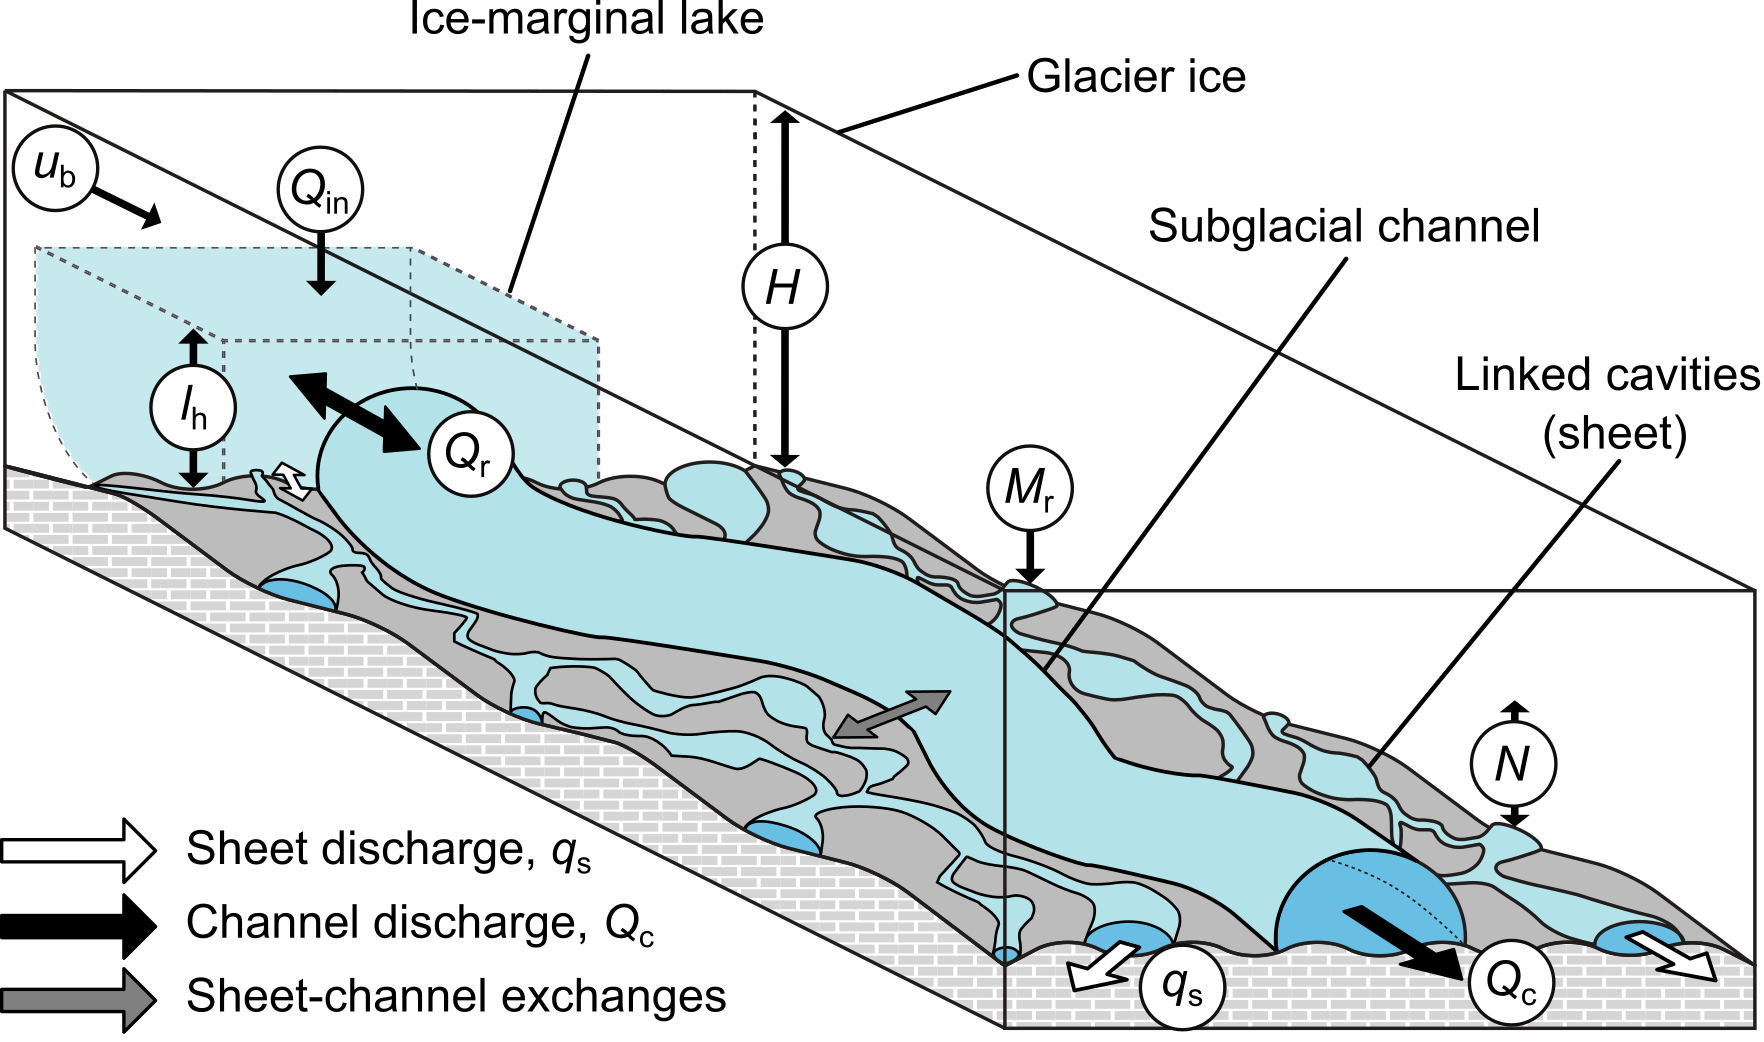
\includegraphics[width=0.45\textwidth]{./figures/Figure_1/Figure_1.png}}
\caption{Schematic illustration of our model, showing a glacier (with thickness, $H$) and ice-marginal lake (with height, $l_{\mathrm{h}}$, and input, $Q_{\mathrm{in}}$). The lake is connected two-ways to a subglacial channel (with discharge, $Q_{\mathrm{c}}$) and a `sheet' of linked cavities (with discharge $q_{\mathrm{s}}$) fed by a basal melt term ($M_{\mathrm{r}}$). Changes in $l_{\mathrm{h}}$ modifies $Q_{\mathrm{s}}$ and $q_{\mathrm{s}}$ which in turn changes basal velocity, $U_{\mathrm{b}}$ through effective pressure, $N$. Note, although the ice-marginal lake is shown as connected to one channel, in our model an ice-marginal lake can be connected to the subglacial system at multiple outlets. \texttt{[SINGLE-COLUMN]}}
\label{FIG:1}
\end{figure}


\subsection{Ice Flow and subglacial drainage models}\label{methods:GlaDS}

We used the GlaDS model \citep{werder2013modeling} as integrated into ISSM \citep{larour2012continental}. GlaDS itself is a widely used (REF) 2D continuum model of subglacial hydrology. We refer interested readers to Appendix~\ref{Appendix:GlaDS} for an overview of key GlaDS equations, and to \cite{werder2013modeling} for a full description of the equations governing water flow. In summary, GlaDS operates on an anisotropic mesh generated using ISSM and includes a description of i) distributed flow through a series of linked cavities represented as a continuous sheet with variable thickness, and ii) channelised flow through Röthlisberger channels that are represented along element edges. Sheet elements exchange water with channels, and the cross-sectional area of these channels evolves through time due to the dissipation of potential energy, sensible heat exchange, and cavity closure rates due to viscous ice creep. Discharge in both the distributed ($q_{\mathrm{s}}$, $\mathrm{m}^2 \mathrm{s}^{-1}$) and channelised system ($Q_{\mathrm{c}}$, $\mathrm{m}^{3} \mathrm{s}^{-1}$) is driven by gradients in the hydraulic potential, $\nabla \phi$ ($\mathrm{Pa}\,\mathrm{m}^{-1}$), with steeper hydraulic gradients driving enhanced water discharge. In GlaDS, $Q_{\mathrm{c}}$ is always non-zero along every internal edge, though only a few reach a discernible discharge. For ease of visualisation we follow previous work [REF] in declaring edges where $Q_{\mathrm{c}} \geq$1 m$^3$s$^{-1}$ to be `meaningful channels' (e.g., Fig.~\ref{FIG:2}c--e, Fig.~\ref{FIG:5}c, Fig.~\ref{FIG:6}--e). ISSM is a finite element higher-order ice-flow model which operates on anisotropic meshes and can be fully-coupled to additional modelling components \citep{larour2012continental}. In addition to the ice-marginal lake modifications, which we describe below (Section~\ref{methods:Lake}), the primary difference between the original GlaDS \citep{werder2013modeling} and the ISSM version used here is thatrather than assuming water flow within the sheet to always be turbulent \citep[cf:][]{werder2013modeling}, we make use of the \cite{hill2024improved} transition parametrisation, whereby sheet flow switches between laminar and turbulent flow according to the local Reynolds number.


%In addition to the ice-marginal lake modifications which we describe below (Section~\ref{methods:Lake}), we note two key differences between the original GlaDS \citep{werder2013modeling} and the ISSM version used here: i) rather than assuming water flow within the sheet to always be turbulent \citep[cf:][]{werder2013modeling}, we make use of the \cite{hill2024improved} transition parametrisation, whereby sheet flow switches between laminar and turbulent flow according to the local Reynolds number, and ii) following \cite{stevens2022tidewater}, we implemented a viscously deforming `elastic sheet layer' which crudely represents hydraulic jacking where water pressure exceeds ice overburden pressure (see Section~\ref{Appendix:GlaDS}). 

To capture the influence of ice-marginal lake drainage on ice dynamics, we include a two-way coupling between ice flow and subglacial hydrology. The GlaDS derived effective pressure ($N=p_{\mathrm{i}}-p_{\mathrm{w}}$, where $p_{\mathrm{i}}$ is ice pressure and $p_{\mathrm{w}}$ is water pressure, $Pa$) modifies basal velocity $U_{\mathrm{b}}$ ($\mathrm{m}\, \mathrm{a}^{-1}$)by governing frictional resistance at the ice-bed interface. In turn, the magnitude of $U_{\mathrm{b}}$ modifies the rate at which cavities open and thereby controls the thickness of the sheet (Eq.~\ref{appeqn: hs_cav}--\ref{appeqn: basal sliding}*). Two-way coupling between ISSM and GlaDS is a relatively new development, and the influence of friction parameters remains the subject of ongoing research \citep[e.g.,][ADD MORE REF]{khan2024inland}, though model response is known to be strongly influenced by the choice of friction law \citep{choi2023impact}. We view this work as necessarily explorative [Flesh this out more], and we do not undertake a full analysis of the modelling interactions between subglacial hydrology and ice dynamics, which is beyond the scope of this work. Rather, we seek to capture the broad influence ice-marginal lake drainage cycles have upon ice dynamics. Accordingly, we present results using two widely applied friction laws: i) the `Budd-style' friction law [REF] implemented in ISSM in terms of basal stress with the form:

\begin{equation}
\label{eq:frictionBudd}
\begin{aligned}
\tau_{\mathrm{b}} = C^{2}_{\mathrm{b}} N^{\mathrm{r}} U_{\mathrm{b}}^{s} ,
\end{aligned}
\end{equation}

where $\tau_{\mathrm{b}}$ is the basal stress magnitude (UNITS), $C_{\mathrm{b}}$ is the friction coefficient, $N$ is effective pressure, $U_{\mathrm{b}}$ is basal velocity magnitude, and both $r$ and $s$ are friction coefficients, or ii) a Schoof-style friction law [REF] with the form: 

\begin{equation}
\label{eq:frictionSchoof}
\begin{aligned}
\tau_{\mathrm{b}}=\frac{C_{\mathrm{s}}^2 v_{\mathrm{b}}^m}{\left(1+\left(\frac{C_{\mathrm{s}}^2}{C_{\max } N}\right)^{1 / m} U_{\mathrm{b}}\right)^m},
\end{aligned}
\end{equation}

where $C_{\mathrm{s}}$ is the \textit{Schoof} friction coefficient, $m$ is a friction law exponent, and $C_{\mathrm{max}}$ is Iken's bound. 





\subsection{Lake evolution}\label{methods:Lake}

Following \cite{kingslake2013modelling} lake depth, $l_{\mathrm{h}}$ ($\mathrm{m}$, Fig.~\ref{FIG:1}), evolves according to the continuity equation:


\begin{equation}
\label{eq:lakecontinuity}
\begin{aligned}
\frac{\mathrm{d} l_{\mathrm{h}}}{\mathrm{d} t} = \frac{1}{A_{\mathrm{L}}}[Q_{\mathrm{in}}-Q_{\mathrm{r}}(t-1)],
\end{aligned}
\end{equation}
\noindent
where $A_L$ is the uniform lake area ($\mathrm{m}^2$), $Q_{\mathrm{in}}$ ($\mathrm{m}^3 \mathrm{s}^{-1}$) represents extraglacial lake input (e.g., rainfall, surface runoff) and $Q_{\mathrm{r}}$ ($\mathrm{m}^3 \mathrm{s}^{-1}$) represents inflow/outflow at the lake outlet(s) from the previous timestep. In moving from a 1D to 2D representation of subglacial hydrology we include the contribution from the sheet, so that $Q_{\mathrm{r}}$ in our model is given by:

\begin{equation}
\label{eq:sumQr}
\begin{aligned}
Q_{\mathrm{r}}(t) = \sum_{i=1}^{n} \left( q_{\mathrm{s},i}(t) + Q_{\mathrm{c},i}(t) \right),
\end{aligned}
\end{equation}
\noindent
or the sum of the width integrated sheet discharge, $q_{\mathrm{s}}$, and channel discharge, $Q_{\mathrm{c}}$ along $n$ vertices connected to an ice-marginal lake. In GlaDS, a specific hydraulic potential is prescribed at outlets (Dirichlet boundary conditions), which is typically equivalent to zero water pressure \citep[i.e., atmospheric pressure, ][]{werder2013modeling}. As a boundary condition at lake outlets, hydrostatic lake pressure fixes the lake outlet hydraulic potential, $\phi_{\mathrm{outlet}}$ to be: 

\begin{equation}
\label{eq:lakephi}
\begin{aligned}
\phi_{\mathrm{outlet}}(t) = \rho_{\mathrm{w}}gz_{\mathrm{b}} + \rho_{\mathrm{w}}gl_{\mathrm{h}}(t) ,
\end{aligned}
\end{equation}

at all times, where $g$ is gravitational acceleration ($\mathrm{m}\,\mathrm{s}^{-1}$) and $z_{\mathrm{b}}$ is bed elevation ($\mathrm{m a.s.l}$). The evolving $\phi_{\mathrm{outlet}}$ handles the coupling between subgalical hydrology and ice-marginal lake by modifying the local $\nabla \phi$ and therefore changing sheet/channel discharge (see Eq.~\ref{appeqn:gladsqs} \&~\ref{appeqn: Qc}).

\subsection{Method of numerical solution}\label{methods:Numeric}

We solve for $l_{\mathrm{h}}$ using a Picard fixed-point iteration scheme comprising an outer and inner loop. In the outer loop, we update $l_{\mathrm{h}}$ given $Q_{\mathrm{r}}$ from the previous timestep (Eqn.~\ref{eq:lakecontinuity}) using a backward Euler solver and use this to set $\phi_{\mathrm{outlet}}$ (Eqn.~\ref{eq:lakephi}) at the current timestep. In the inner loop, GlaDS solves for the domain-wide $\phi$ until it satisfies a set convergence criteria, as in previous implementations of GlaDS \citep[see:][]{werder2013modeling,hill2024improved}. Following the inner loop converging, and given the global $\phi$, the model updates $h_{\mathrm{s}}$, $N$,$Q_{\mathrm{c}}$, and $q_{\mathrm{s}}$, before summing $Q_{\mathrm{c}}$ and $q_{\mathrm{s}}$ at lake outlet nodes to give $Q_{\mathrm{r}}$ (Eqn.~\ref{eq:sumQr}). The outer loop iterates until the norm of the current and previous $l_{\mathrm{h}}$ satisfies a given tolerance. 

\begin{table}
\begin{minipage}{86mm}
\footnotesize
\caption{Variables and Units\protect\footnotemark}
\label{tab:Var}
\begin{tabular}{@{}ccc}
\hline
Variable & Units & Description \\
\hline
$\phi$ & Pa & Hydraulic potential \\
$Q_{\mathrm{c}}$ & m$^{3}$s$^{-1}$ & Channel discharge \\
$q_{\mathrm{s}}$ & $\mathrm{m}^{2}\,\mathrm{s}^{-1}$ & Sheet discharge \\
$h_{\mathrm{s}}$ & m & Sheet thickness\footnote{Note this includes the elastic sheet and cavity sheet thickness, see Eq.~\ref{appeqn: hs_el}--\ref{appeqn: hs_cav}} \\
$l_{\mathrm{h}}$ & m & Lake Height \\
$Q_{\mathrm{r}}$ & m$^{3}$s$^{-1}$ & Lake discharge \\
$U_{\mathrm{b}}$ & $\mathrm{m\,a}^{-1}$ & Magnitude of basal velocity\\
$u_{\mathrm{b}}$ & $\mathrm{m\,a}^{-1}$ & x-component of basal velocity \\
$v_{\mathrm{b}}$ & $\mathrm{m\,a}^{-1}$ & y-component of basal velocity \\
$S$ & $\mathrm{m}^2$ & Channel cross-sectional area \\
\hfill \\
$t$ & yrs & Time coordinate \\
$X$ & km & Horizontal coordinate \\
$Y$ & km & Vertical coordinate \\
\hfill \\
\hfill \\
$N$ & Pa & Effective pressure \\
\hline
\end{tabular}

\footnotetext{The first section lists dependent variables, the second section lists coordinates, and the third section lists derived variables [FIX ORDER.]}

\end{minipage}
\end{table}


\section{Model application to a synthetic domain}\label{application:synth}

We test our model on a simple 10$\times$3 km rectangular domain (Figure~\ref{FIG:2}c--f), discretised on a 2D triangular mesh with a characteristic edge length of 100 m ($n_{\mathrm{vertices}}$=2486). The bed elevation, $h_{\mathrm{b}}$ is characterised by a gentle slope ($\sin=0.0075$) dipping towards the terminus, and ice thickness is parabolic ($H \propto \sqrt{x}$) increasing from from $H$=50 m at $X$= 0 km to $H$ = $\sim$155 m at $X$ = 10 km. A 5 km$^{2}$ ice-marginal lake was connected to a single vertex at the upper boundary of the domain where $(X, Y) = (10,\ 1.5)\ \text{km}$. To facilitate comparison with previous work, our domain is similar in scale and geometry to that in \cite{kingslake2013modelling}, which was chosen to be loosely analogous to the Merzbacher Lake and South Inylchek Glacier, Kyrgyztan \citep{ng2009temporal}. 

Model variables are given in Table~\ref{tab:Var} and our synthetic model parameters are given in Table~\ref{tab:Synth}. The parameter dependency of GlaDS has already been extensively explore elsewhere [REF]. To efficiently explore the parameter dependence of our ice-marginal lake drainage model we limited our testing to those previously highlighted as critical to subglacial drainage (e.g., channel/sheet conductivity terms, $k_{\mathrm{c}}$/$k_{\mathrm{s}}$, the basal bump height, $h_{\mathrm{b}}$, the channel sheet width, $l_{\mathrm{c}}$, and the cavity spacing, $l_{\mathrm{r}}$) as well as the terms which control the input of water into both the subglacial system (basal melt rate), and the ice-marginal lake (lake refill rate, $Q_{\mathrm{in}}$). As is common-practice, we varied one parameter at a time between a minimum and maximum bound (Table~\ref{tab:Synth}) informed both by previous work [REF] and the limits of numerical stability. As reference, an additional simulation was taken as the approximate midpoint of each of these parameters (Fig.~\ref{FIG:3}). Each simulation was run for a total of 15 years and had a 30 minute timestep. We used a Budd-style friction law (Eq.~\ref{eq:frictionBudd}) with the coefficient $C_{\mathrm{b}} = 100$ and exponents $r = 1/4$ and $s = 1/4$. The ice dynamic model was initialised with $U_{\mathrm{b}} = 100,\mathrm{m,a}^{-1}$, with Dirichlet boundary conditions ($U_{\mathrm{b}} = 0,\mathrm{m,a}^{-1}$) at the terminus and stress-free Neumann boundary conditions elsewhere. The hydrology model was initialised with $\phi$ equivalent to 90\% of ice overburden pressure, and an initial sheet thickness, $h_{\mathrm{s}}$ equal to half the bump height, $h_{\mathrm{b}}$. We prescribe $\phi$ terminus $X = $0 km to be $\approx$1$\times$10$^{4}$ as our GlaDS Dirichlet boundary condition, though arbitrary, this does not qualitatively affect our results below. We impose zero water inflow as our Neumann boundary condition at the other three boundaries. The ice-marginal lake had an initial height of 30 m ($l_{\mathrm{h}}$ at $t$=0). The evolution of the reference case through time is shown in Fig.~\ref{FIG:2}, and the sensitivity of lake height ($l_{\mathrm{h}}$), flood discharge ($Q_{\mathrm{r}}$), and basal velocity magnitude ($U_{\mathrm{b}}$) through time is shown in Figs.~\ref{FIG:3} \&~\ref{FIG:4}).

\begin{table}
\footnotesize
%\begin{minipage}{86mm}
\begin{minipage}{172mm}
\footnotesize
\caption{Input parameters in our synthetic domain. The parameters we varied are highlighted in bold, with the reference case value given first and the range over which they varied in parentheses.}
\label{tab:Synth}
\begin{tabular}{@{\,\,\,}l@{\,\,\,}c@{\,\,\,}c@{\,\,\,}c@{\,\,\,}}

\hline
Description & Symbol & Value(s) & Units \\
\hline
Gravitational acceleration & $g$ & 9.81 & m s$^{-1}$ \\
Latent heat & $L$ & 3.34$\times$10$^{5}$ & J kg$^{-1}$ \\
Ice density & $\rho_{\mathrm{i}}$ & 917* & kg m$^{-3}$ \\
Freshwater density & $\rho_{\mathrm{w}}$ & 1000 & kg m$^{-3}$ \\
Pressure melt coefficient & $c_{\mathrm{t}}$ & 7.5$\times$10$^{-8}$ & K Pa$^{-1}$ \\
Heat capacity of water & $c_{\mathrm{w}}$ & FOLLOW UP & J kg$^{-1}$K$^{-1}$ \\
Glen's $n$ & $n$ & 3 & \hfill \\
Ice flow constant at the bed\footnote{The bed is assumed to be at pressure melting point, but the ice column is assumed equivalent to -10$^{\degree}$C or $A=$4.9$\times$10$^{-25}$ Pa$^{-n}$s$^{-1}$} & $A_{b}$ & 6.8$\times$10$^{-24}$ & Pa$^{-n}$s$^{-1}$ \\
%\hfill \\
Bed elevation & $z_{\mathrm{b}}$ & \hfill & m \\
Ice thickness & $H$ & \hfill & m \\
%\hfill \\
Budd friction coefficient & $C_{\mathrm{b}}$ & 100 & \\ 
First friction law exponent & $r$ & 1/4 & \hfill \\
Second friction law exponent & $s$ & 1/4 & \hfill \\
%\hfill \\
Channel conductivity & $k_{\mathrm{c}}$ & \textbf{0.1 (0.2--0.01)} & m$^{\frac{3}{2}}$kg$^{-\frac{1}{2}}$ \\
Sheet conductivity\footnote{Note that following \cite{hill2024improved} the units for $k_{s}$ differ from those given by \cite{werder2013modeling}} & $k_{s}$ & \textbf{0.02 (0.05--0.005)} & Pa s$^{-1}$ \\
Englacial void ratio & $e_{\mathrm{v}}$ & 1$\times$10$^{-4}$ & \hfill \\
First sheet flow exponent & $\alpha_{\mathrm{s}}$ & 5/4 & \hfill \\
Second sheet flow exponent & $\beta_{\mathrm{s}}$ & 3/2 & \hfill \\
First channel flow exponent & $\alpha_{\mathrm{c}}$ & 5/4 & \hfill \\
Second channel flow exponent & $\beta_{\mathrm{c}}$ & 3/2 & \hfill \\
Transition parameter & $\omega$ & 1/2000 & \hfill \\
Basal bump height & $h_{\mathrm{b}}$ & \textbf{0.1 (0.2--0.05)} & m \\
Channel sheet width & $l_{\mathrm{c}}$ & \textbf{20 (50--5)} & m \\
Cavity spacing & $l_{\mathrm{r}}$ & \textbf{5 (20--1)} & m \\
Basal melt rate & $M_{\mathrm{r}}$ & \textbf{0.25 (5--0.1)} & m a$^{-1}$ \\
Lake refill rate & $Q_{\mathrm{in}}$ & \textbf{10 (20--5)} & m$^{3}$s$^{-1}$ \\
Elastic sheet depth scale & $h_{\mathrm{c}}$ & 0 & m \\
Elastic sheet exponent & $\gamma$ & 1 & \hfill \\
Uplift regularisation rate & $h_{\varepsilon}$ & 1$\times$10$^{-6}$ & m Pa$^{-1}$ \\
Regularising pressure & $N_{\varepsilon}$ & 1$\times$10$^{4}$ & Pa \\
\hline
\end{tabular}
\end{minipage}
\end{table}

\subsection{Stable flood cycles}

In our reference case, the ice-marginal lake undergoes recurrent, stable, and asymmetric lake filling and draining cycles (Fig.~\ref{FIG:2}a). Likewise, each lake filling and draining cycle is associated with a recurring flood with stable maximum amplitude and duration (Fig.~\ref{FIG:2}b). The lake only partially drains each flood cycle, and never reaches a height necessary to sustain flotation ($N$=0, Fig.~\ref{FIG:2}f). For the initial 5 years of the simulation, as the model adjusts to initial conditions, peak flood discharge increases with each successive flood, and the lake reaches successively lower post-flood lowstands (Fig.~\ref{FIG:2}a,b). Thereafter, the flood cycles reach a stable periodicity (Fig.~\ref{FIG:2}f) and clockwise hysteresis with flood cycles occurring approximately every 1.5 years.  

The evolution of the subglacial channel system through a single flood cycle is shown in Fig.~\ref{FIG:2}c--e (an animated version is shown in SUPP MOVIE), and the width-averaged basal velocity response over the same flood cycle and into the following is shown in Fig.~\ref{FIG:2}g. At the start of a flood cycle (Fig.~\ref{FIG:2}c), as the lake approaches its highstand, the system is characterised by limited channelised drainage and $\nabla\phi$ generally perpendicular to the ice surface slope. Close to the lake outlet ($X > \mathrm{9 km}$), contours of hydraulic potential appear concave forming a `ridge' at the lake outlet. In GlaDS, sheet discharge, $q_{\mathrm{s}}$, is directed perpendicular to these contours and such ridges indicate sheet flow out of the lake. Four short ($<$100 m), low-discharge ($\leq$1 m$^{3}\mathrm{s}^{-1}$ channels remain open following the previous flood cycle, three at the terminus and one connected to the lake outlet.

During the lake filling phase, increasing $l_\mathrm{{h}}$ drives $\phi_{\mathrm{outlet}}$ up (Eq.~\ref{eq:lakephi}), resulting in a steeper $\nabla \phi$ across the domain and promoting channelised drainage close to the lake outlet [SUPP MOVIE]. During the lake drainage phase, initiated once $Q_{\mathrm{r}}$ begins to rapidly exceed the lake refill rate, $Q_{\mathrm{in}}$ (when $l_\mathrm{{h}} \approx \mathrm{75\ m}$ and $t \approx \mathrm{7.9 yrs}$) an arborescent channel structure originating from the lake outlet extends across the full-width of the domain, perpendicular to the contours of $\phi$, and therefore offset to the direction of ice-surface slope. Simultaneously, channels extend upglacier from the terminus, and contours of $\phi$ become increasingly convex. At the flood peak channel tributaries coalesce into the three primary terminus channels which evacuate water from the system. As the lake level drops sharply during a flood, $\phi_{\mathrm{outlet}}$ drops, reducing $\nabla \phi$, and in turn reducing $Q_{\mathrm{c}}$ below the level necessary to sustain channels across the domain, including at the lake outlet. Once $Q_{\mathrm{r}} < Q_{\mathrm{in}}$ the flood terminates and the cycle begins anew. Each cycle takes $\approx$1.5 years with the exponentially rising and falling limb of the flood lasting $\approx$6 months. 

Basal velocity, $U_{\mathrm{b}}$ changes significantly throughout a flood cycle and tracking the development of a significant channelised drainage system (e.g., Fig.~\ref{FIG:2}g). Our synthetic glacier gradually accelerating during the flood initiation phase before channelised drainage is widely established, then abruptly decelerating $\approx$two months before the flood peak (Fig.~\ref{FIG:2}g) once channels are well established. Ice flow acceleration propagates from the lake outlet towards the terminus, with maximum velocity sustained within 2 km of the lake outlet. 


%\clearpage
\begin{figure}
\centering{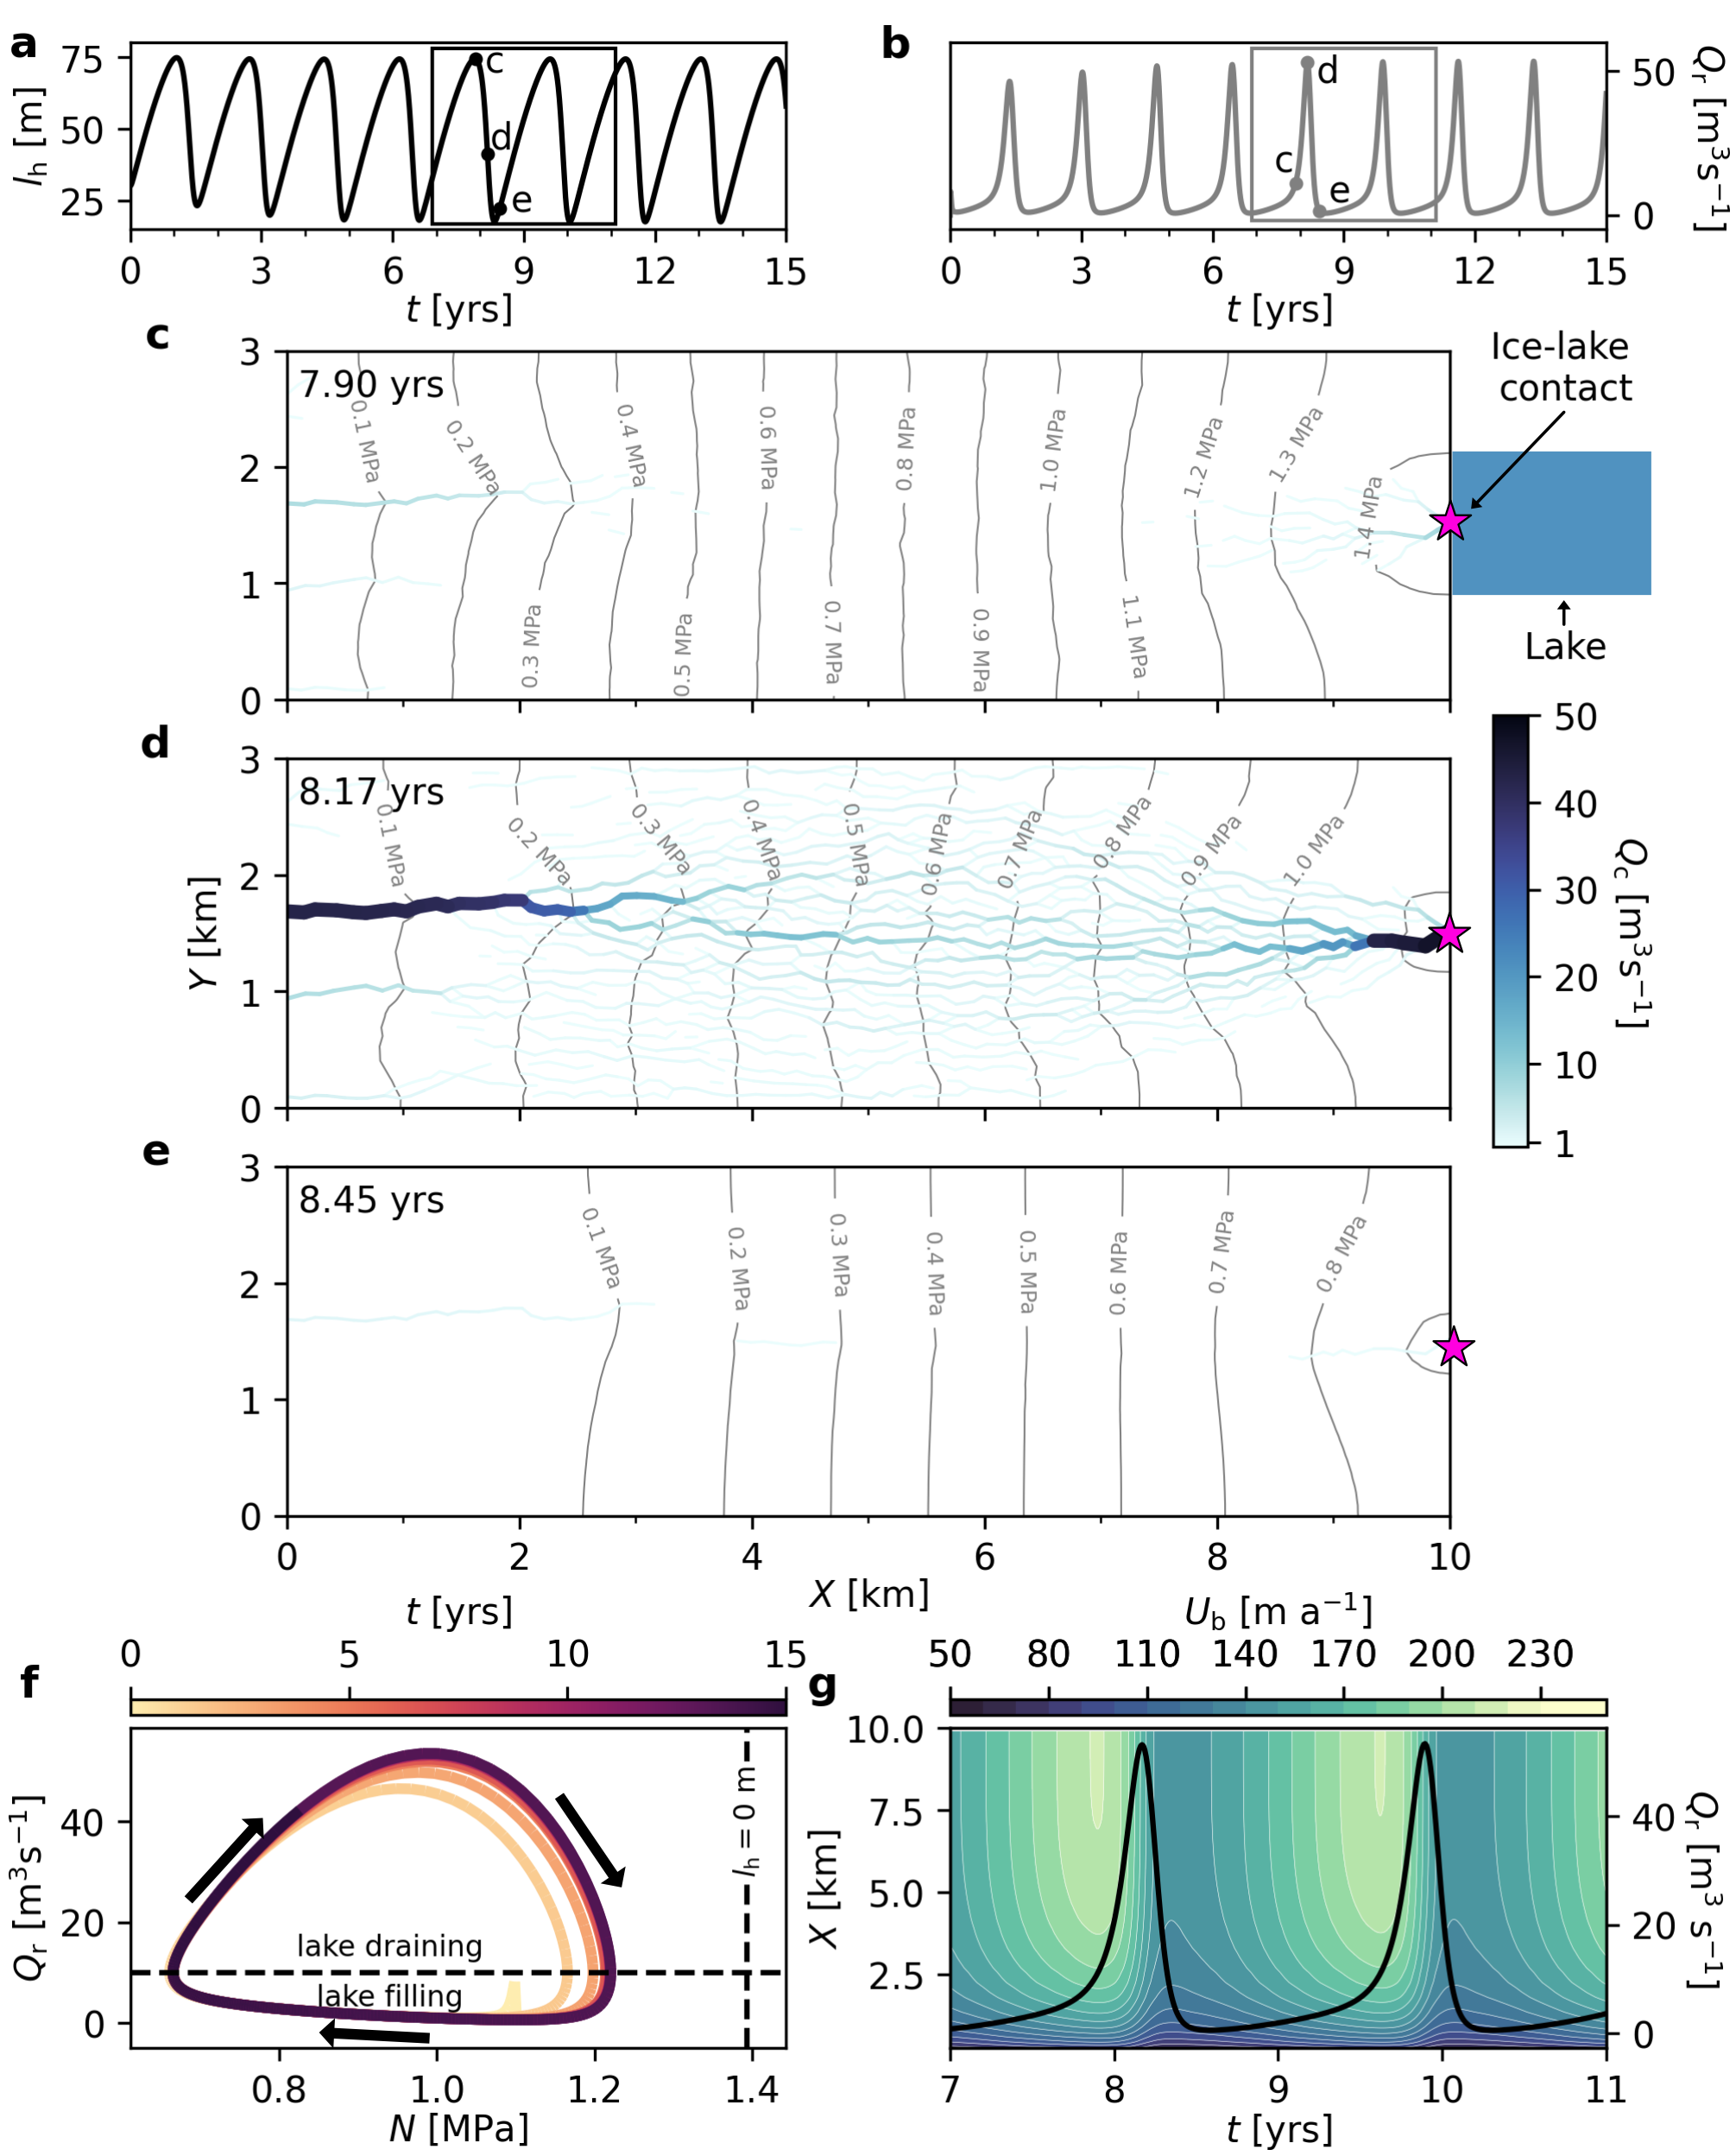
\includegraphics[width=0.95\textwidth]{./figures/Figure_2/Figure_2.png}}
\caption{Evolution of the 'reference' model configuration in our synthetic modelling domain. \textbf{a}) Lake height, $l_{\mathrm{h}}$ through time. Black points indicate $l_{\mathrm{h}}$ in panels \textbf{c}--\textbf{e}. \textbf{b}) Sum discharge at the lake outlet, $Q_{\mathrm{r}}$ through time. Grey points indicate $Q_{\mathrm{r}}$ in panels \textbf{c}--\textbf{e} the grey box indicates the time span of panel \textbf{g}. \textbf{c}--\textbf{e}) Channel discharge, $Q_{\mathrm{c}}$ at $t=$7.10 years (\textbf{c}), 8.38 years (\textbf{d}) and 9.00 years (\textbf{e}). In each panel, effective pressure, $N$ is shown as grey contours and the lake outlet is marked by a magenta star. \textbf{f}) Phase-plane diagram showing the evolution of $Q_{\mathrm{r}}$ and $N$ through time at the ice-marginal lake outlet. Arrows and shading indicate the direction of time. The horizontal dashed line denotes the lake refill rate, $Q_{\mathrm{in}} =$ 10 m$^{3}$s$^{-1}$. The vertical dashed line indicates $N$ when $l_{\mathrm{h}}=$0 m. \textbf{g}) Filled contour plot showing the across-flow averaged velocity through time. White contours represent velocity (every 10 ma$^{-1}$) and the black line shows $Q_{\mathrm{r}}$ between years 7--11.}
\label{FIG:2}
\end{figure}
%\clearpage
%\addtocounter{figure}{-1}
%\noindent\captionof{figure}{test}



\subsection{Parameter sensitivity}


Fig.~\ref{FIG:3} shows the time series from a total of 14 simulations across the maximum (red lines), minimum (blue lines) parameter values with the reference `\textit{mid-point}' simulation in grey. The majority of simulations yield stable and recurring asymmetric lake filling and drainage cycles (Fig.~\ref{FIG:3}a[i]--f[i]) with corresponding floods in channel discharge at the lake outlet, $Q_{\mathrm{r}}$ (Fig.~\ref{FIG:3}a[ii)]--f[ii]). Amongst the parameters tested, the clearest influence is on the amplitude of lake height and its rate of change, both of which in turn influence the timing of flood initiation and peak flood discharge, with higher amplitude flood cycles leading to higher peak flood discharges.

Increasing channel conductivity, $k_{\mathrm{c}}$, in effect making channels more sensitive to $\nabla \phi$ (see Eq.~\ref{appeqn: Qc}), leads to lower lake highstands, higher peak discharge and total lake drainage. At maximum $k_{\mathrm{c}}$, the model takes longer to reach a fixed flood return interval, draining at a higher frequency than the default case until $\sim \ \\mathrm{years}$ into the simulation at which point flood cycles occur at approximatley the same interval as in the default case. Conversely, at minimum $k_{\mathrm{c}}$, the capacity of channels to drain the lake is inhibited and flood onset is delayed. Because channels grow slowly, peak $Q_{\mathrm{r}}$ is also dampened leading to relatively long flood cycle durations ($\sim \ 5\ \mathrm{years}$).

Increasing the sheet conductivity, $k_{\mathrm{s}}$ increases the capacity of the sheet to accommodate water and delays transmission to channels, this results in reduced lake highstands and delayed flood initiation as the onset of classical channel growth is delayed. Reducing $k_{\mathrm{s}}$ increases the relative efficiency of channels and leads to more vigorous lake-fill drain cycles, which shorter and more intense floods as a result. Changing $h_{\mathrm{b}}$ has a similar effect to reducing $k_{\mathrm{s}}$, although at the maximum bump height, the sheet becomes so efficient that it can accommodate all lake discharge and within 1 year the lake reaches a stable equilibrium where $Q_{\mathrm{r}} = Q_{\mathrm{in}}$. 

Changing the contributing width of the sheet to the channel ($l_{\mathrm{c}}$) or the representative horizontal spacing of cavities ($l_{\mathrm{r}}$) has similar influence on lake drainage by altering the relative efficiency of channelised and sheet drainage. Reducing $l_{\mathrm{r}}$ and increasing $l_{\mathrm{c}}$ reduces the amplitude of lake height and lowers peak discharge, and vice versa when increasing $l_{\mathrm{r}}$ and reducing $l_{\mathrm{c}}$. 

Finally, increasing input of water into the either the glacier via basal melt rate, $M_{\mathrm{r}}$ or lake via $Q_{\mathrm{in}}$ enhances the amplitude of $l_{\mathrm{h}}$ oscillations and in turn peak flood discharge. 

In all simulations, the maximum lake height remains below the maximum ice thickness and does not surpass the effective pressure $N=0$ necessary to initiate ice flotation. In the majority of simulations the lake lowstand does not fall below $\sim$10 m, only draining completely when $k_{\mathrm{c}}$ = 0.25 m$^{\frac{3}{2}}$kg$^{-\frac{1}{2}}$, and when $h_{\mathrm{b}}=0.05\ \mathrm{m}$.

%\clearpage
\begin{figure}
\centering{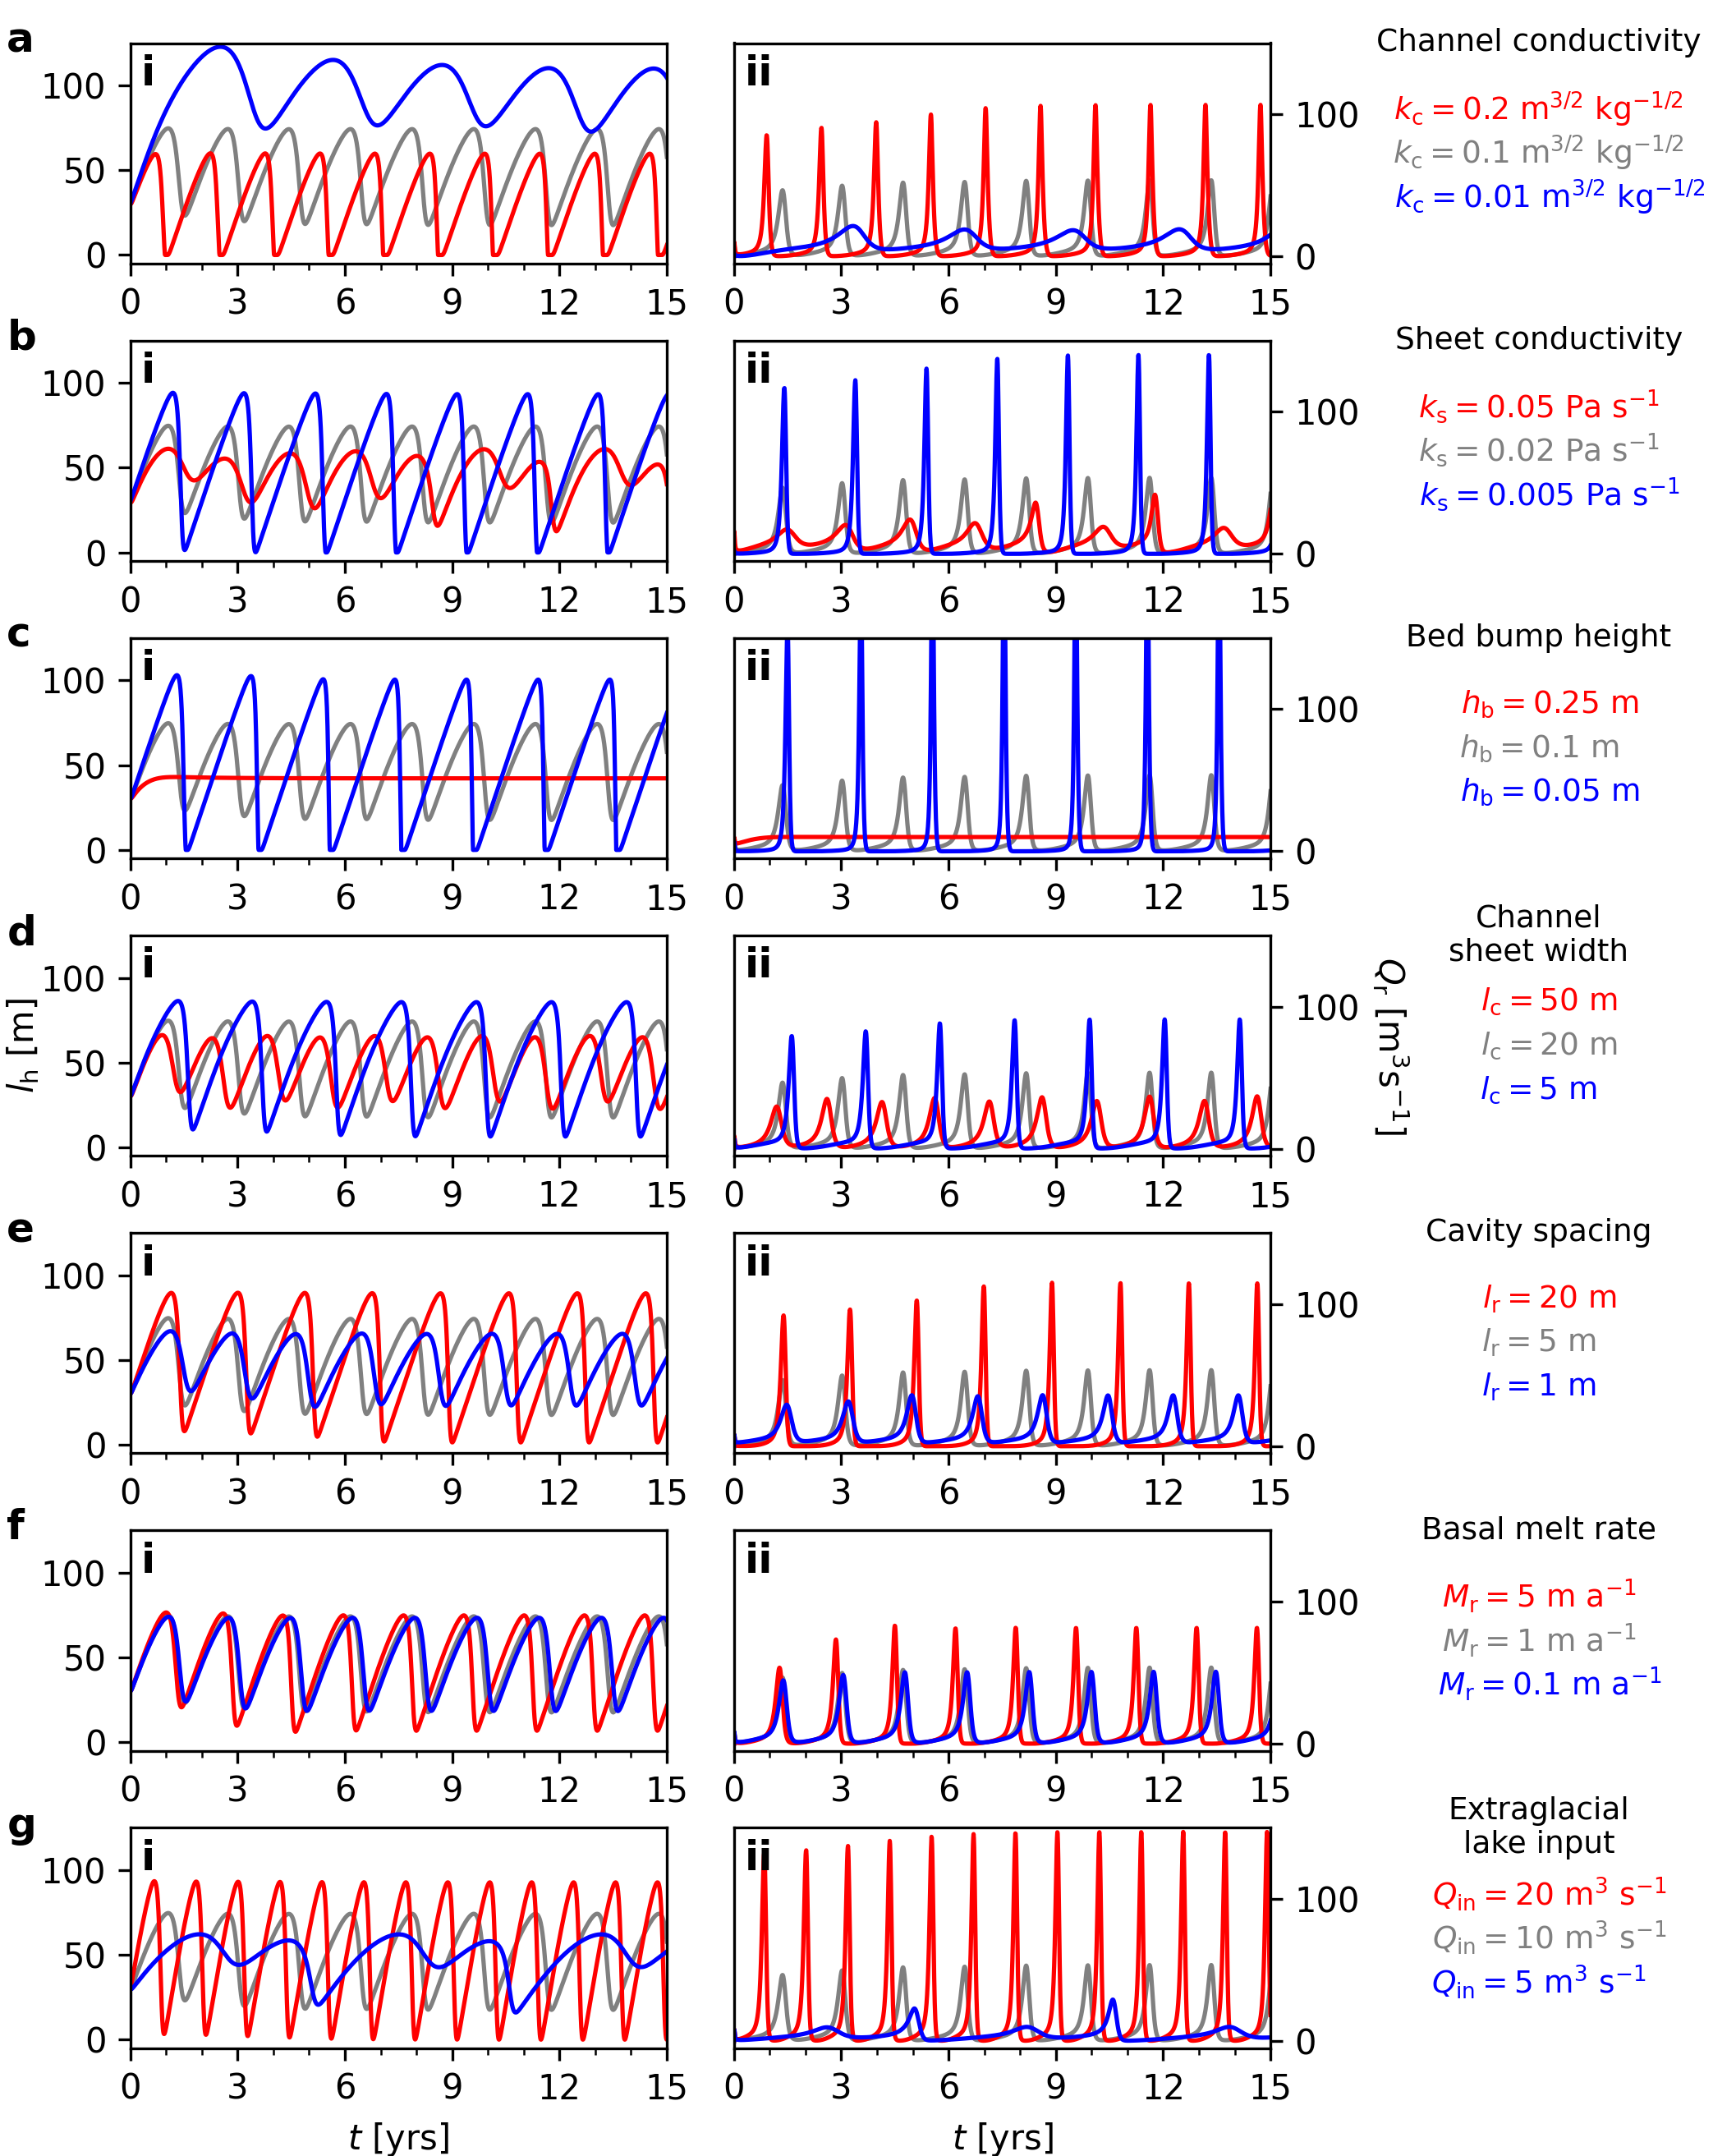
\includegraphics[width=0.95\textwidth]{./figures/Figure_3/Figure_3.png}}
\caption{Lake height, $l_{\mathrm{h}}$ (left panels, i) and sum discharge at the lake outlet, $Q_{\mathrm{r}}$ (right panels, ii) across a range of key model parameters. \textbf{a}) Channel conductivity, $k_{\mathrm{c}}$. \textbf{b}) Sheet conductivity, $k_{\mathrm{s}}$. \textbf{c}) Basal bump height, $h_{\mathrm{b}}$. \textbf{d}) Channel sheet width, $l_{\mathrm{c}}$. \textbf{e}) Cavity spacing, $l_{\mathrm{r}}$. \textbf{f}) Basal melt rate, $M_{\mathrm{r}}$. \textbf{g}) Lake refill rate, $Q_{\mathrm{in}}$. In all panels, the default parameter run is shown in grey.}
\label{FIG:3}
\end{figure}

The characteristics of the lake filling-drainage cycle across our parameter space also strongly influences the resulting basal velocity signal, and Figure~\ref{FIG:4} shows the width-averaged velocity during at least one complete flood cycle for $k_{\mathrm{c}}$, $k_{\mathrm{s}}$, and $h_{\mathrm{b}}$. Each model follows the reference case with velocity peaking before peak discharge is reached, and dropping rapidly thereafter along the falling limb of a flood. In general, shorter more intense flood cycles lead to a more rapid and higher magnitude velocity response, whereas more broad and less intense flood cycles yield a similar velocity response, maintaining peak velocity for a longer duration. However, the highest basal velocity ($>300 \mathrm{m a}^{-1}$) is associated with the low $k_{\mathrm{c}}$ case (Fig.~\ref{FIG:4}), characterised by muted lake filling-drainage cycles but a relatively high lake-level (Fig.~\ref{FIG:3}a[i]). 


\begin{figure}
\centering{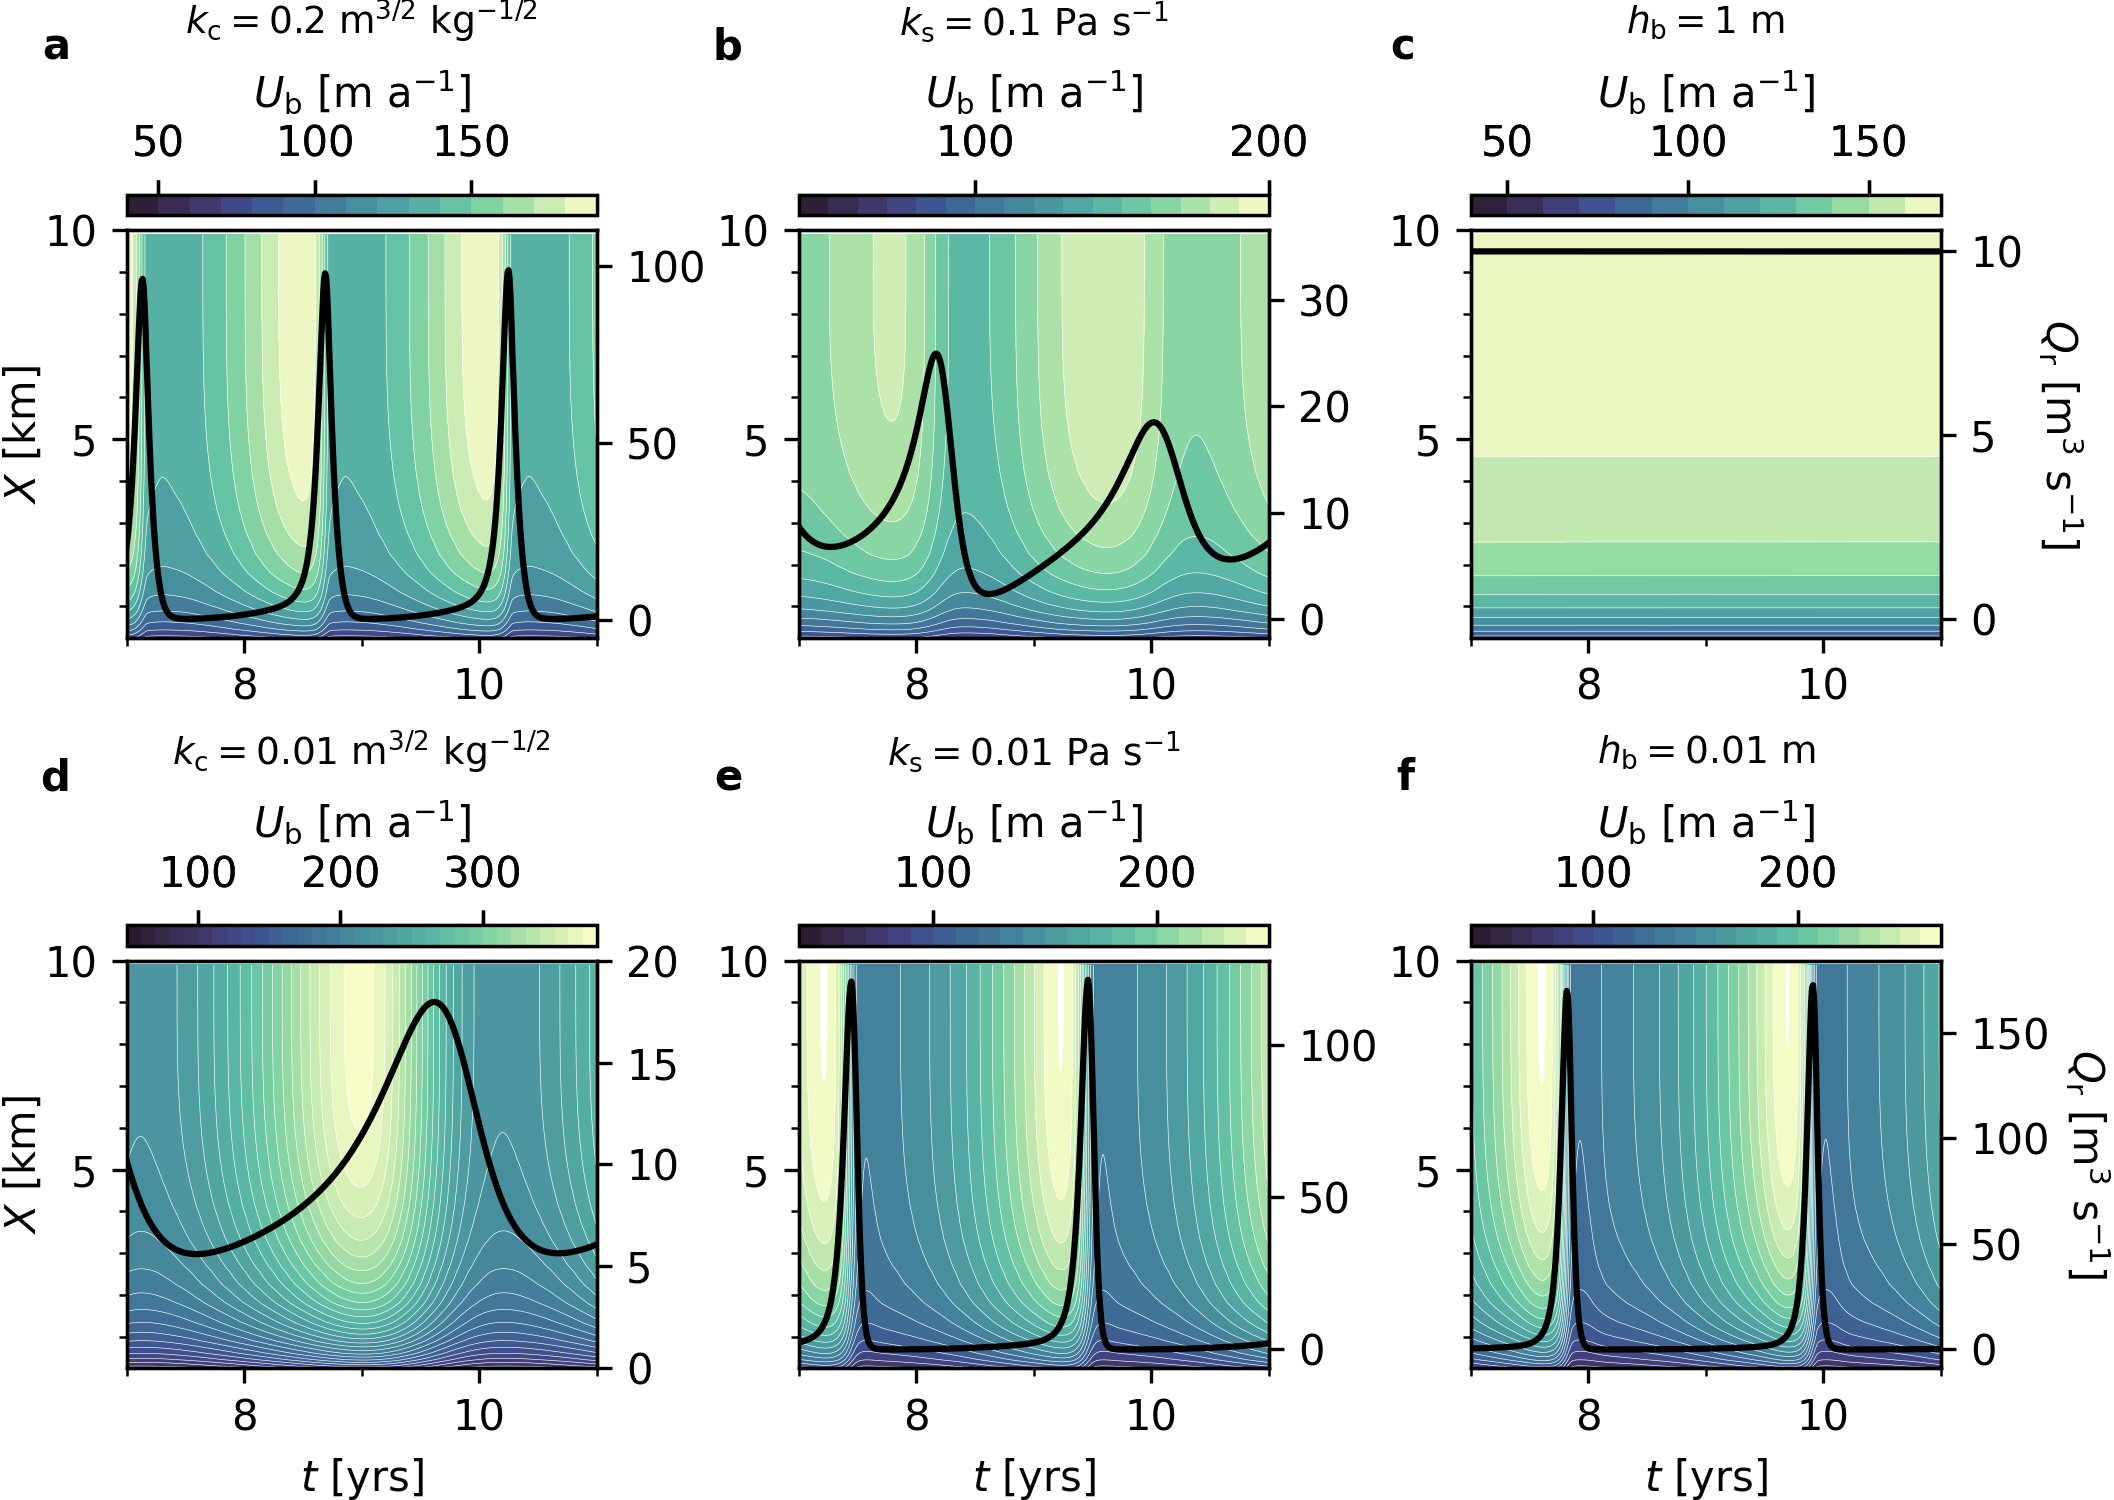
\includegraphics[width=0.95\textwidth]{./figures/Figure_4/Figure_4.png}}
\caption{Across-flow velocity through time for key GlaDS parameters in the synthetic experiment. \textbf{a--c}) The high channel conductivity ($k_{\mathrm{c}}$, a), sheet conductivity ($k_{\mathrm{s}}$, b), and bump height ($h_{b}$, c) cases. \textbf{d--e}) The low $k_{\mathrm{c}}$ (d), $k_{\mathrm{s}}$ (e), and $h_{b}$ (f) cases. In each panel, white contours represent velocity (every 10 ma$^{-1}$) and the black line shows $Q_{\mathrm{r}}$ between years 7--11.}
\label{FIG:4}
\end{figure}

\section{Model application to a real domain}\label{application:greenland}


We applied our model to Isunnguata Sermia, an outlet glacier in West Greenland draining a catchment of  $\approx\!16\,000\ \mathrm{km}^2$. The central drainage axis of Isunnguata Sermia is characterised by a deep, flow-parallel trough with an anabranching structure in its upper reaches. A recently described  $\approx\!3\ \mathrm{km}^2$, $\approx\!100\ \mathrm{m}$ deep ice-dammed lake \citep{livingstone2025ice} abuts the northern margin of Isunnguata Sermia's tongue. The lake drains subglacially with a periodicity of 1--3 years, undergoing at least 12 fill-drain cycles between 1987--2024 \citep[][Fig.~\ref{FIG:5}f]{livingstone2025ice}. There are two ice-contact boundaries between Isunnguata Sermia and the ice-marginal lake, a prominent boundary along the western margin of the lake through which the lake appears to drain, and an intermittent boundary along the eastern margin that is established once lake level is sufficiently high \citep{livingstone2025ice}.

\subsection{Model setup} \label{application:setup}

% Field data, including passive seismics, GNSS, and time-lapse imagery is available for one drainage in 2023 \citep[see; ][]{livingstone2025ice}. 

We discretised our Isunnguata Sermia domain (Source of original catchment?) using an anistropic mesh with an edge length of 150 m close to terminus, increasing to 2 km close to the upper margin of our domain at the approximate ELA (at \( H \approx 1600\ \text{m} \)). The mesh was further refined to a typical edge length of 50 m close to the lake outlets (Fig.~\ref{FIG:5}b,c). Bedmachine v5 was used for $z_{\mathrm{b}}$ and $H$ \citep[][Fig.~\ref{FIG:5}b,c]{Morlighem_Et_Al_2022}. An initialisation $U_{\mathrm{b}}$ was taken from the 2021 MEaSUREs annual mosaic \citep{MEASURES}, from which we inverted for the basal friction coefficient using an L-curve scheme \citep[following; ][]{wolovick2023regularization}. Because we have an observational constraint on ice-surface velocity, we used a Schoof-style friction law (see Eq.~\ref{eq:frictionSchoof}, Section~\ref{methods:GlaDS}) which has been shown to more faithfully represent ice-dynamics with a GlaDS derived $N$ than the Budd-style friction law used in our synthetic experiments \citep{mcarthur2023basal}. Geothermal heat flux was taken from \citep{shapiro2004inferring}, basal melt rates were taken from \cite{karlsson2021first} and surface ice temperature was taken from \citep{ettema2009higher}. The flow-law rate factor $A$ within the ice-column was derived using these surface ice temperatures and assuming a temperature-dependent Arrhenius relation following \cite{cuffey2010physics}.

As boundary conditions to our hydrology solution, we imposed Dirichlet conditions along the western and eastern margins of the lake, as well as at the glacier terminus. Neumann (zero-inflow) conditions were imposed elsewhere. Along the western lake margin (where the glacier is always in contact with the lake), we fixed bed elevation equal to the minimum lake elevation (257.9 m a.s.l) at seven vertices, and at the eastern margin we identified the lowest elevation vertex within a group of vertices close to the observed stream and fixed this at 257.9 m. At each lake outlet (magenta stars in Fig.~\ref{FIG:4}), $\phi_\mathrm{outlet}$ was allowed to evolve with $l_{\mathrm{h}}$ (equation~\ref{eq:lakephi}). Because the lake model is spatially lumped and cannot dynamically represent intermittent lake–glacier contact along the eastern margin, prescribing the same boudary conditions here as along the western lake boundary provides a simple and consistent boundary treatment and ensures subglacial channel discharge is fed into the ice-marginal lake. At the glacier terminus we prescribe $\phi$ equal to atmospheric pressure at the lowest elevation boundary vertex (cyan triangle in Fig.~\ref{FIG:5}c). Within the ice-dynamic solution, the boundary velocity is given by the initialisation $U_{\mathrm{b}}$ (Dirichlet), except at the western lake margin where velocity is allowed to evolve freely (Neumann). 

As climate forcing, we used the 10 km resolution daily Modèle Atmosphérique Régional (MAR, v3.14) runoff and accumlation data \citep{fettweis2017reconstructions} between 2007--2025. In the synthetic test case, we kept $Q_{\mathrm{in}$ fixed through time, however the rate of lake refill is likely to be variable in time as a function of air-temperature and climate \citep{ng2009temporal}. To account for this, we use a simple temperature index \citep[as in][]{kingslake2015chaotic}, where $Q_{\mathrm{in}}$ is given by: 


\begin{equation}
\label{eq:Tempindex}
\begin{aligned}
Q_{\mathrm{in}} =
\begin{cases}
kT, & T > 0 \\
1, & T \le 0
\end{cases}
\end{aligned}
\end{equation}

where the temperature-index coefficient $ k $ is equal to $2\mathrm{m}^{3}\mathrm{s}^{-1}\mathrm{K}^{-1}$. We set $Q_{\mathrm{in}} > 1$ to capture positive changes in lake elevation observed between melt seasons in Fig~\ref{FIG:5}f. Our Greenland-specific GlaDS parameters, those which differ from in the synthetic case, are given in Table~\ref{tab:Synth}. 

Our experimental approach was split into two phases, the first of which was to obtain a basal friction coefficient $C$. We ran an initial inversion for $C$ using an empirically-derived $N$ taking into account bed topography and ice thickness, before running a simple GlaDS-only model run over 10 years, which did not include an ice-marginal lake, surface melt or two-way coupling to ice dynamics. This allowed us to derive a more realistic and spatially variable $N$ from which a second inversion for basal friction could be obtained. Such an approach has previously been demonstrated to yield more faithful basal inversions in a coupled hydrology model \citep[see;][]{ehrenfeucht2023seasonal,mcarthur2023basal}. 

Our primary model phase, in which we ran our model for a total of 38 years with a 5 minute timestep, consisted of a `steady state' phase, followed by a `spin-up' into a full transient simulation. In the steady state phase, we ran our model for 20 years, until the 95\textsuperscript{th} percentile difference in sheet thickness between successive timesteps fell below $1\times10^{-6} \mathrm{m}$. During the steady state phase, we allowed the ice-marginal lake to freely evolve from an initial height of $l_{\mathrm{h}}=70\ \mathrm{m}$, or the mean lake height between 1987--2024 \citep{livingstone2025ice}. The steady state phase allowed the model to reach a condition which approximates the anticipated wintertime hydrological conditions in which there is limited channel activity and water pressures across the domain are close to the flotation fraction ($p_{\mathrm{w}}\approx 0.7-0.9 p_{\mathrm{i}}$). In the transient phase, taking the results of the steady-state run as initial conditions, we spun our model up over 10 years with a climate forcing that was gradually introduced by increasing the 2007 runoff by 10\% each year. Following this spin-up, the full transient simulation proceeded from 2007 onwards using the MAR timeseries until the end of 2025.



\begin{figure}
\centering{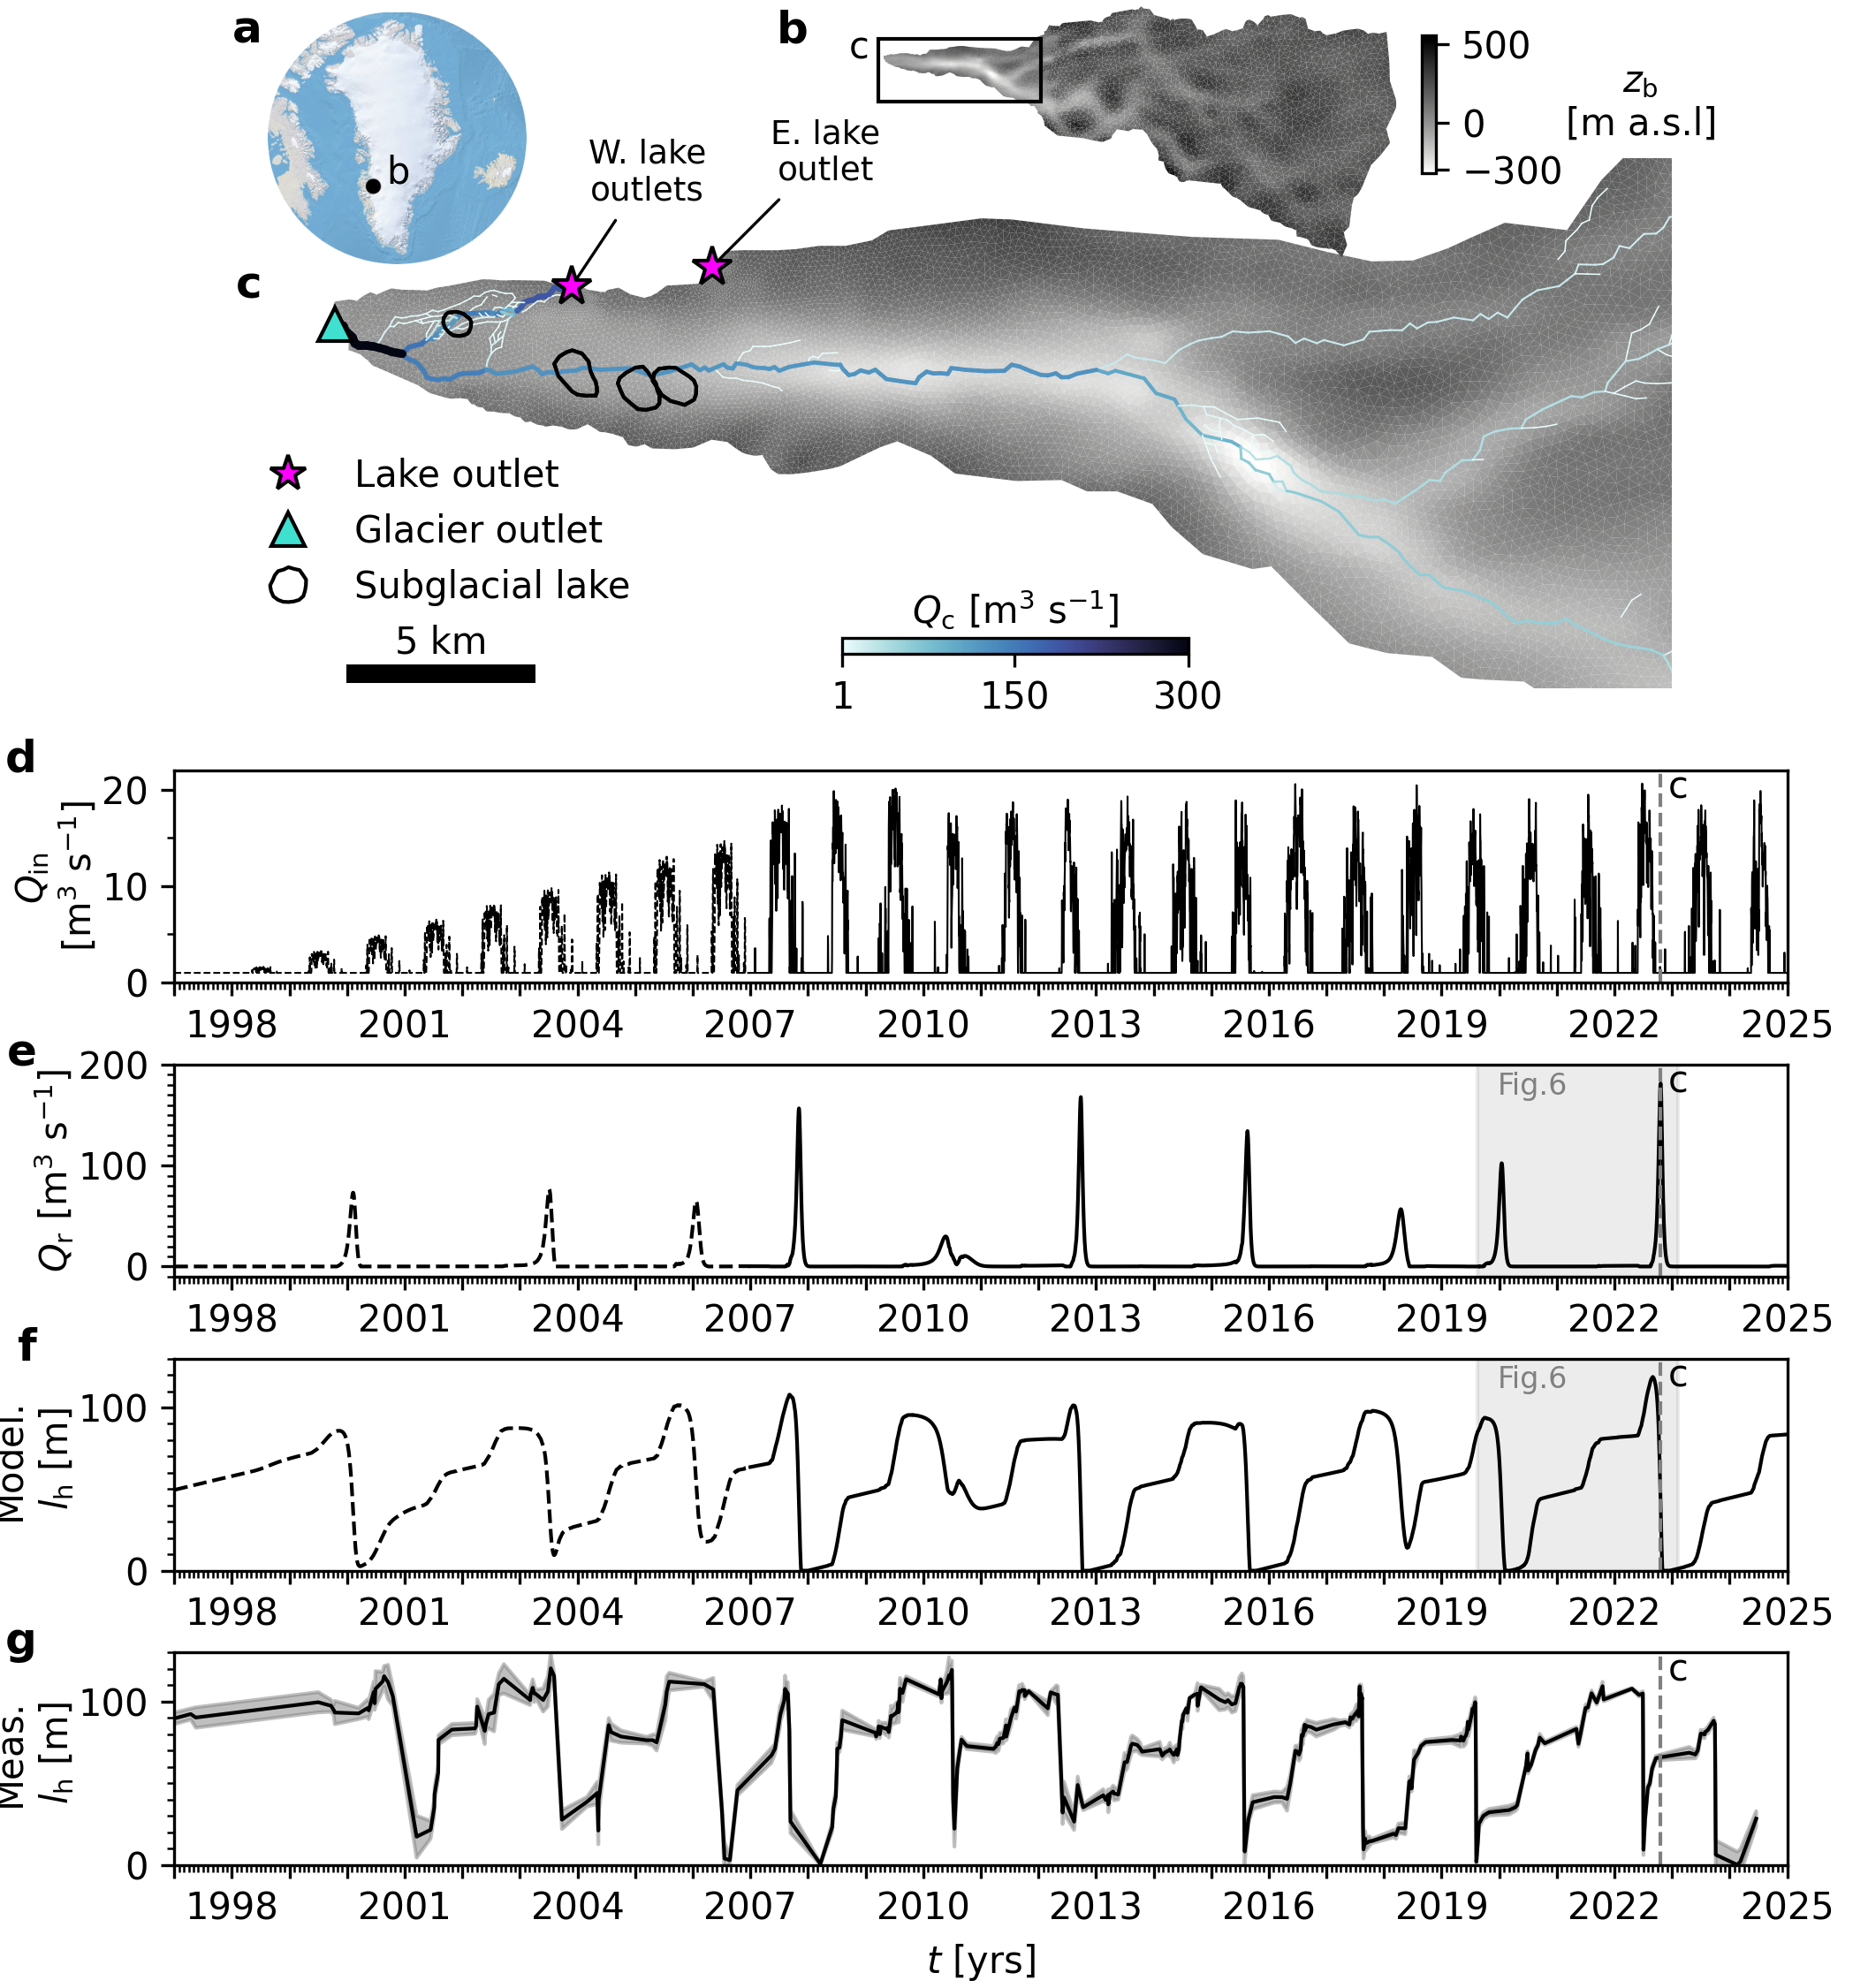
\includegraphics[width=\textwidth]{./figures/Figure_5/Figure_5.png}}
\caption{Ice-marginal lake drainage in the Isunnguata Sermia glacier catchment. \textbf{a}) the location of our model domain (panel b) in southwest Greenland. \textbf{b} our modelling domain, coloured by the bed elevation \citep{Morlighem_Et_Al_2022}, the extent of panel c is outlined. \textbf{c}) channel discharge, $Q_{\mathrm{c}}$ at the end of the 2018 melt season. The primary drainage axes is located within the along-flow orientated subglacial trough. The location of the lake outlets and the glacier outlets are marked by a pink star and a cyan triangles respectively The location of subglacial lakes 0--3 discussed in \cite{livingstone2025ice} are shown in black polygons. \textbf{d}) 95$^{th}$ percentile runoff during the spinup (dashed line) and transient modelling phase (solid line). Runoff increases by 10\% each year during the spin-up phase (1997--2007). \textbf{e}) sum outlet discharge, $Q_{\mathrm{r}}$ at the lake outlets during the spinup (dashed line) and transient modelling phase (solid line). Values lower than zero indicate net discharge into the lake, and vice versa when $Q_{\mathrm{r}} > 0$.\textbf{f}) modelled lake height, $l_{\mathrm{h}}$ during the spinup (dashed line) and transient modelling phase (solid line). \textbf{g}) Measured $l_{\mathrm{h}}$ and uncertainty values taken from \cite{livingstone2025ice}. The dashed vertical line in panels d--f shows the time represented by panel c, and the shaded grey box indicates the time span shown in Fig~\ref{FIG:6}.} 
\label{FIG:5}
\end{figure}

\subsection{Flood cycles in West Greenland} \label{application:results}


The full primary phase of our Greenland simulation is shown in Fig~\ref{FIG:5}. The spin-up phase (dashed line in Fig~\ref{FIG:5}d--f) is characterised by three cycles of lake filling and partial drainage, each of which reach successively higher lake highstands and have a shorter return period than the flood prior, tracking the development of a catchment wide sub-glacial drainage system together with successively more intense melt summers (Fig~\ref{FIG:5}d). From 2007 onwards, once the model is subject to the full extent of annual melt-forcing, the lake repeatedly fills and drains with a recurrence interval between floods of $\sim$2--4 years. As in the synthetic case, lake fill and drainage cycles are characterised by a gradual lake filling phase and a rapid lake drainage phase, though the signal is notably more complex. Lake drainages typically occur at the end of a melt season. Lake levels then remain low during the subsequent winter, before filling in a stepwise fashion, with the lake filling more rapidly during summer melt seasons and remaining stable, or lowering slightly, during the intervening winter period. Lake drainage is triggered following the second or third melt season, and the cycle begins anew. 

The timing of lake 



Though variable in peak discharge and duration, a flood will typically commence with the development of 

The velocity pattern 

\begin{figure}
\centering{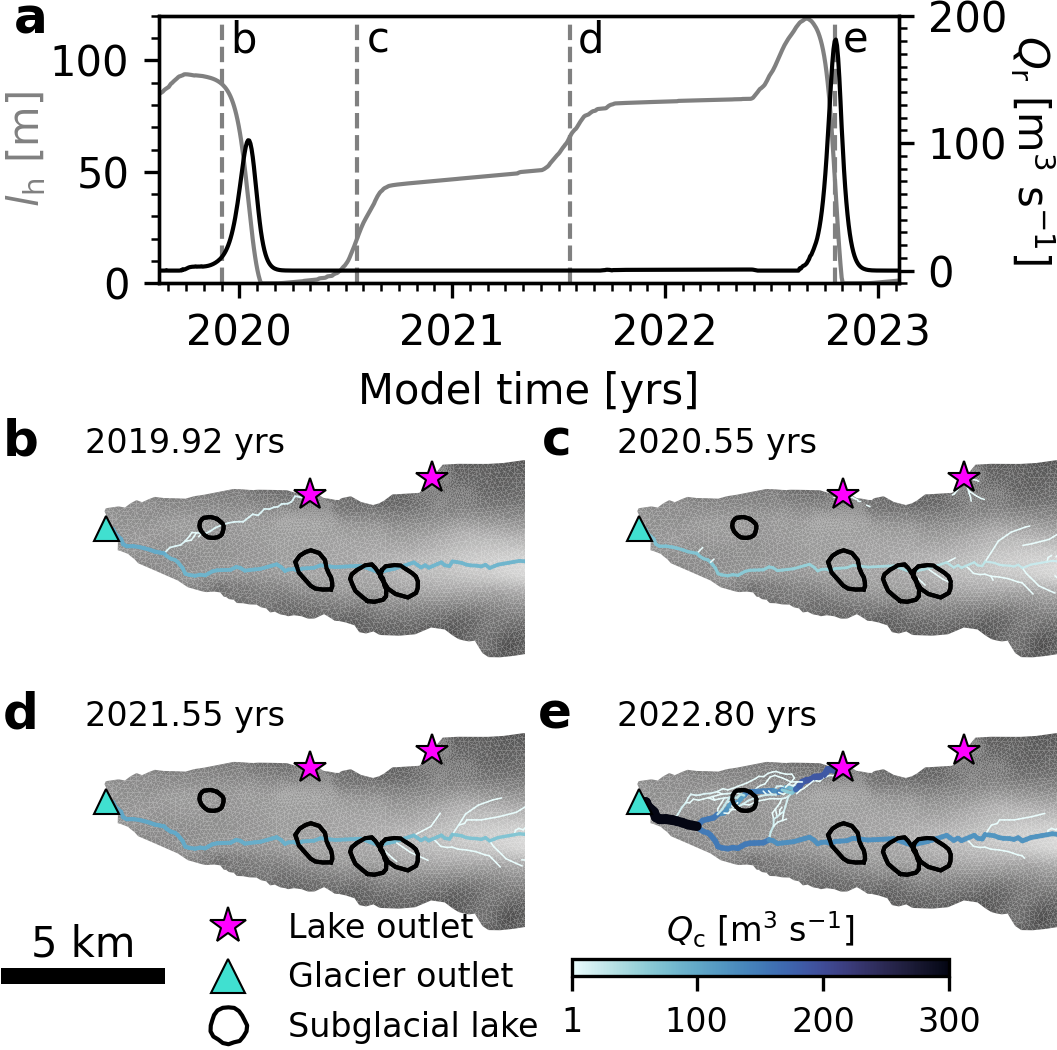
\includegraphics[width=0.45\textwidth]{./figures/Figure_6/Figure_6.png}}
\caption{Channel development during a complete lake filling--drainage cycle. \textbf{a}) lake height, $l_{\mathrm{h}}$ and flood outlet discharge, $Q_{\mathrm{r}}$ through time. \textbf{b--e}) snapshots of channel discharge, $Q_{\mathrm{c}}$ through time, with the location of lake outlets and the glacier outlet marked by pink stars and a cyan triangle respectively. The location of subglacial lakes 0--3 discussed in \cite{livingstone2025ice} are shown in black polygons. Dashed lines in panel a indicate the snapshot times in panels b--e. [SINGLE-COLUMN] }
\label{FIG:6}
\end{figure}



\begin{table}
\begin{minipage}{86mm}
\caption{Parameters in our Greenland run, listing those which differ from Table~\ref{tab:Synth}}
\label{tab:Greenland}
\begin{tabular}{@{}ccc}
\hline
Variable & Units & Description \\
\hline
\hline
\end{tabular}

\end{minipage}
\end{table}

\section{Discussion} 

\begin{figure}
\centering{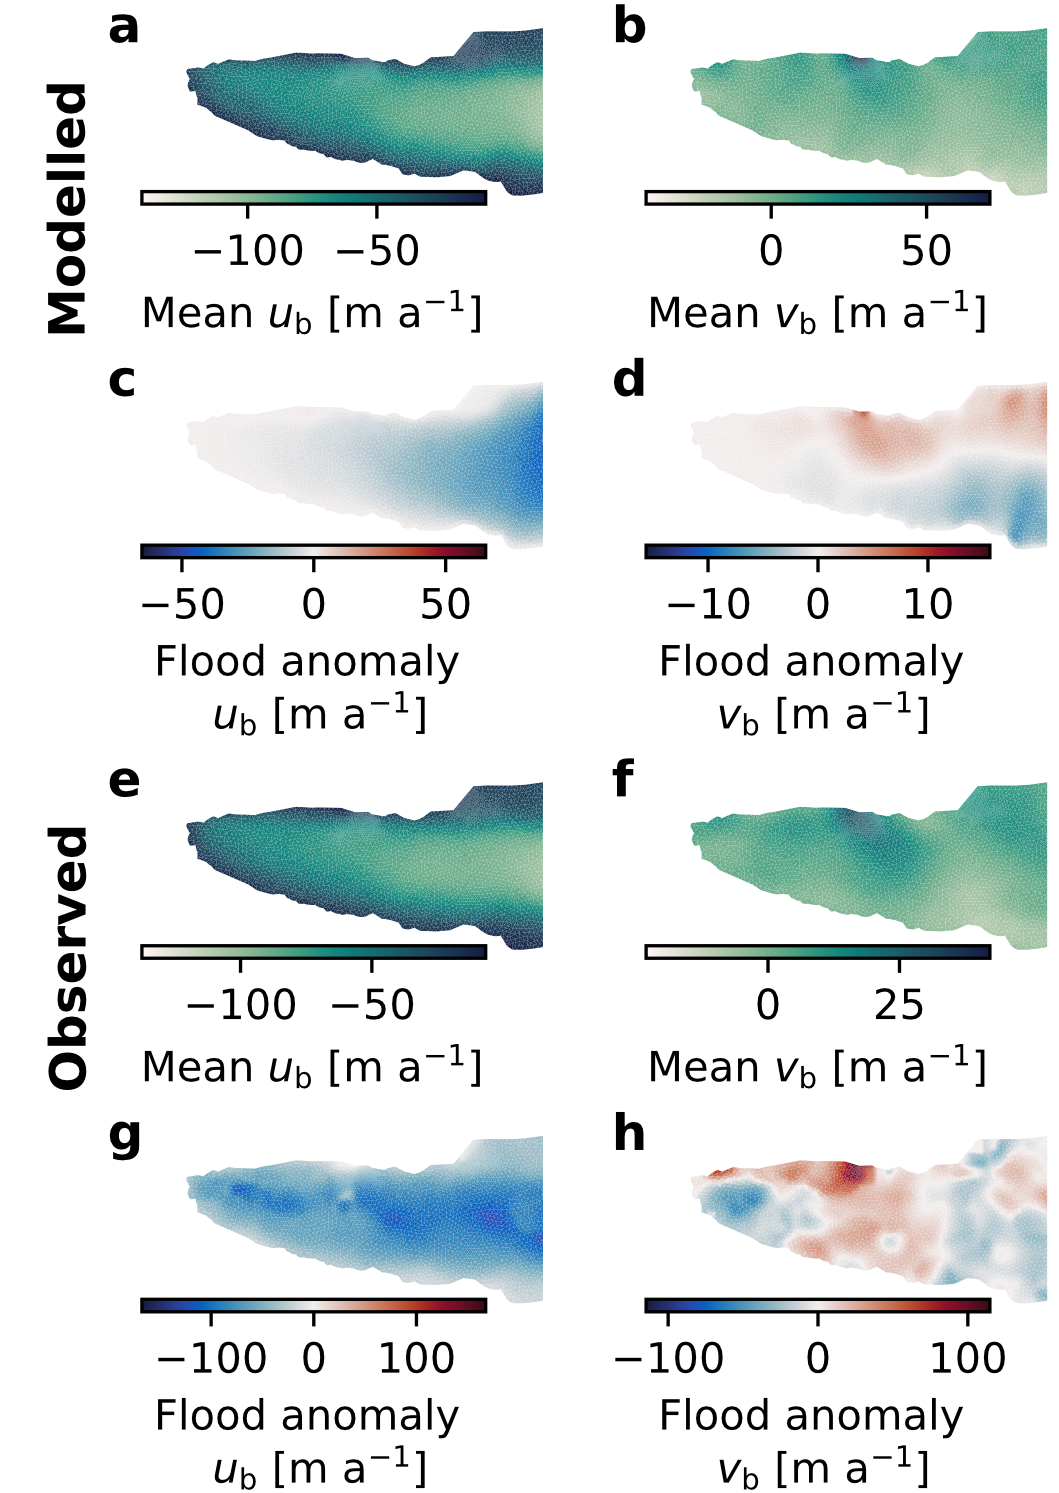
\includegraphics[width=0.45\textwidth]{./figures/Figure_7/Figure_7.png}}
\caption{Comparison of modelled (a--d) and observed (e--h) velocity during a lake drainage. \textbf{a--b}) Mean modelled velocity components, $u_{\mathrm{b}}$ (a) and  $v_{\mathrm{b}}$ (b), for the model years 2014--2025. \textbf{c--d}) Anomalies in velocity components, $u_{\mathrm{b}}$ (c) and  $v_{\mathrm{b}}$ (d), during the modelled 2018 lake drainage (see Fig~\ref{FIG:5} \& \ref{FIG:6}. \textbf{e--f}) Mean observed velocity components, $u_{\mathrm{b}}$ (e) and  $v_{\mathrm{b}}$ (f), between 2014--2025. \textbf{g--h}) Anomalies in velocity components, $u_{\mathrm{b}}$ (g) and  $v_{\mathrm{b}}$ (h), during an observed lake drainage in 2023 (see Fig~\ref{FIG:5}g). Lake drainage anomalies (c--d \& g--h) calculated by subtracting mean velocity components (2014--2025) from the mean velocity components during a lake drainage event, red colours indicate higher velocity during the lake drainage and blue colours indicate slower velocity. Observed velocity components estimated from Sentinel-1a and Sentinel-1b Synthetic  Aperture  Radar  (SAR), see \cite{livingstone2025ice} for details.}
\label{FIG:7}
\end{figure}




\begin{itemize}
\item model reproduces 1) many observed characteristics of Jokulhlaup theory, 2) matches well with Felix and Jonny's work, and 3) successfully reproduces many of the characteristics of IS flooding

\item However it is not perfect, initial conditions are a key uncertainty, as well as the other physically uncertain GlaDS parameters, noting we only carried out a partial sweep here, others were run but had limited influence on drainage characteristics . Something akin to Tim's Gaussian GP emulation might offer a way to more rapidly test the parameter space and select an optimum starting condition. 

\item Future work 


\end{itemize}

\section{Conclusions}








\section{Author contribution statement}

The research was conceptualised by A. Hepburn, S. Buzzard, A. Sole, and S. Livingstone. A. Hepburn developed the model, carried out the experiments, and prepared the analysis. A. Hepburn wrote the manuscript, with input from S. Buzzard, A. Sole, and S. Livingstone. All authors reviewed and edited the manuscript, and fieldwork to deploy and maintain the sensors was carried out by everyone other than A. Hepburn. T. Irvine-Fynn is thanked for his assistance producing Figure 1. Fellowship funding was acquired by A.Hepburn and project funding by S. Livingstone, R. Storrar, S. Buzzard, A. Sole, [FINISH].

\section{Acknowledgements} 

A.J.H is funded by an Aberystwyth University Independent Research Fellowship. Work carried out as part of the NERC-funded SLIDE project (grant No. NE/X000257/1, awarded to S.L). 

\section{Proper nouns will be corrected in references pre-submission...}


% authors generating their own bbl file would uncomment the following two lines, and comment out/delete the references below:

\bibliography{Jokulhlaup}   % reads igsrefs.bib
\bibliographystyle{igs}  % imposes IGS bibliography style on output


\appendix
\section{Additional model description}\label{Appendix:MODEL}

\setcounter{equation}{0}
\renewcommand\theequation{A\arabic{equation}}

\subsection{The Glacier Drainage System model}\label{Appendix:GlaDS}

As described fully in \cite{werder2013modeling}, the hydraulic potential at the bed, $\phi$, is defined at the bed by: 

\begin{equation}
\label{appeq:GlaDSdirBC}
\begin{aligned}
\phi = \phi_{\mathrm{m}} + p_{\mathrm{w}},
\end{aligned}
\end{equation}

with water pressure, $p_{\mathrm{w}}$, and elevation potential

\begin{equation}
\label{eq:elevationpotential}
\begin{aligned}
\phi_{\mathrm{m}} = \rho_{\mathrm{w}}gz_{\mathrm{b}},
\end{aligned}
\end{equation}

where $\rho_{\mathrm{w}}$ is water density, $g$ is gravitational acceleration and $z_{\mathrm{b}}$ is bed elevation. In turn, effective pressure $N$ is given by: 

\begin{equation}
\label{appeqn}
N = p_{\mathrm{i}}-p_{\mathrm{w}} = \phi_{\mathrm{O}}-\phi,
\end{equation}

where $p_{\mathrm{i}}$ is ice overburden pressure ($p_{\mathrm{i}} = \rho_{\mathrm{i}}gH$) and $\phi_{\mathrm{O}}$ is the overburden potential ($\rho_{\mathrm{O}} = \phi_{\mathrm{m}}+p_{\mathrm{i}}$).

In the original GlaDS \citep{werder2013modeling}, sheet discharge, $q_{\mathrm{s}}$ is given by:

\begin{equation}
\label{appeqn:gladsqs}
\begin{aligned}
q_{\mathrm{s}} = -k_{\mathrm{s}}h_{\mathrm{s}}^{\alpha}|\nabla \phi|^{\beta}\nabla \phi,
\end{aligned}
\end{equation}

where $k_{\mathrm{s}}$ is the sheet conductivity; $h_{\mathrm{s}}$ is the sheet thickness; and $\alpha$ and $\beta$ are flow exponents. Following the Darcy-Weisbach law, when flow is fully turbulent the flow exponents $\alpha=\mathrm{5/4}$ and $\beta=\mathrm{3/2}$. Here we use the \cite{hill2024improved} laminar-turbulent transition model, and with $\alpha_{\mathrm{s}}= \mathrm{5/4}$ as here, Eq~\ref{appeqn:gladsqs} becomes:  

\begin{equation}
\label{appeqn: Transition}
\begin{aligned}
q_{\mathrm{s}} = -\frac{\nu}{2 \omega} \left(\frac{h_{\mathrm{b}}}{h_{\mathrm{s}}}\right)^{1 / 2} \hspace{10em}\\
\hspace{3em} \cdot \left(-1 + \sqrt{1 + 4 \frac{\omega}{\nu} \left(\frac{h_{\mathrm{s}}}{h_{\mathrm{b}}}\right)^{1 / 2} k_{\mathrm{s}} h^3 |\nabla \phi|} \right) \frac{\nabla \phi}{|\nabla \phi|}
\end{aligned}
\end{equation}
where $\omega$ is a laminar–turbulent transition parameter (corresponding to the Reynolds number at which water becomes fully-turbulent), $h_{\mathrm{b}}$ is the bed bump height, and $v$ is the kinematic viscosity of water at 0$^{\degree}$C. 

%In GlaDS, sheet thickness refers to the thickness of the cavity layer only and there is no representation of viscoelastic deformation of the overlying ice once $p_{\mathrm{w}} > p_{\mathrm{i}}$. Here, following \citeauthor{stevens2022tidewater} (\citeyear{stevens2022tidewater}, based on earlier work by \citeauthor{hewitt2013seasonal} \citeyear{hewitt2013seasonal}), we separate the distributed sheet into elastic sheet thickness $h_{\mathrm{el}}$, and cavity sheet thickness $h_{\mathrm{cav}}$, adding them together to give the overall sheet thickness, $h_{\mathrm{s}} = h_{\mathrm{el}} + h_{\mathrm{cav}}$. The elastic sheet thickness is directly related to the water pressure by:

%\begin{equation}
%\label{appeqn: hs_el}
%\begin{aligned}
%h_{\mathrm{el}}=h_c\left(\frac{p_{\mathrm{w}}}{p_{\mathrm{i}}}\right)^\gamma+h_{\varepsilon 2}\left[-N_{-}+\frac{1}{2} %N_{\varepsilon}\left(1-N_{+} / N_{\varepsilon}\right)_{+}^2\right],
%\end{aligned}
%\end{equation}

%where $h_{\mathrm{c}}$ is the elastic sheet depth scale, $\gamma$, is the elastic sheet exponent, $h_{\varepsilon}$ is the uplift regularisation rate, and $N_{\varepsilon}$ is the regularising pressure for uplift regularisation rate. In addition, $N_{-} = \mathrm{min}(N,0)$ and $N_{+} = \mathrm{max}(N,0)$, with the second term designed to increase rapidly once $N<0$, as a basic representation of hydraulic jacking.

The cavity sheet thickness evolves through time given by:

\begin{equation}
\label{appeqn: hs_cav}
\begin{aligned}
\frac{\partial h_{\mathrm{cav}}}{\partial t} = w - r,
\end{aligned}
\end{equation}

for functions $w$ and $r$, which describe the cavity opening and closing rate, respectively \citep{kamb1987glacier,walder1994channelized}. Cavities open at a rate given by basal velocity $U_{\mathrm{b}}$ over basal bumps with height, $h_{\mathrm{b}}$:

\begin{equation}
\label{appeqn: basal sliding}
w(h) = 
	\begin{cases}
	U_{\mathrm{b}}({h_{\mathrm{r}} - h_{\mathrm{s}}})/{l_{\mathrm{r}}} & \text{if } h < h_{\mathrm{r}} \\
	0 & \text{otherwise}
	\end{cases}
\end{equation}

where $l_{\mathrm{r}}$ is the horizontal cavity spacing. Viscous ice deformation leads to cavity closure, related to the effective pressure, $N$ by:

\begin{equation}
\label{appeqn: viscous closure}
\begin{aligned}
r(h,N) = Ah|N|^{n-1}N, 
\end{aligned}
\end{equation}

where $A$ is the rheological constant of ice, multiplied by a first order geometrical factor (h, but double check it is sheet thickness), and $n$ is Glen's flow law exponent. 

Sheet elements exchange water with channels, the cross-sectional of which, $S$, evolve through time due to the dissipation of potential energy, $\Pi$, sensible heat exchange, $\Xi$, and cavity closure rates due to viscous ice creep $v_{\mathrm{c}}$

\begin{equation}
\label{apeq:channel cross section}
\frac{\partial S}{\partial t}=\frac{\Xi-\Pi}{\rho_{\mathrm{i}} L}-v_c,
\end{equation}
\noindent
where $\rho_{\mathrm{i}}$ is the ice density and $L$ is the latent heat of fusion. 

Finally, channel discharge, $Q_{\mathrm{c}}$ is also related to the hydraulic potential gradient by:

\begin{equation}
\label{appeqn: Qc}
\begin{aligned}
Q_{\mathrm{c}} = -k_{\mathrm{c}}S^{\alpha_{\mathrm{c}}}\left|\frac{\partial \phi}{\partial s}\right|^{\beta_{c}-2}\frac{\partial \phi}{\partial s},
\end{aligned}
\end{equation}

where $k_{\mathrm{c}}$ is the channel conductivity; $s$ is the horizontal coordinate along a channel; and $\alpha_{\mathrm{c}}$/$\beta_{\mathrm{c}}$ are channel flow exponents.





\end{document}